%\VignetteIndexEntry{faoswsImputation: A package for the imputation of missing time series data in the Statistical Working System}
%\VignetteEngine{knitr::knitr}
\documentclass[nojss]{jss}\usepackage[]{graphicx}\usepackage[]{color}
%% maxwidth is the original width if it is less than linewidth
%% otherwise use linewidth (to make sure the graphics do not exceed the margin)
\makeatletter
\def\maxwidth{ %
  \ifdim\Gin@nat@width>\linewidth
    \linewidth
  \else
    \Gin@nat@width
  \fi
}
\makeatother

\definecolor{fgcolor}{rgb}{0.345, 0.345, 0.345}
\newcommand{\hlnum}[1]{\textcolor[rgb]{0.686,0.059,0.569}{#1}}%
\newcommand{\hlstr}[1]{\textcolor[rgb]{0.192,0.494,0.8}{#1}}%
\newcommand{\hlcom}[1]{\textcolor[rgb]{0.678,0.584,0.686}{\textit{#1}}}%
\newcommand{\hlopt}[1]{\textcolor[rgb]{0,0,0}{#1}}%
\newcommand{\hlstd}[1]{\textcolor[rgb]{0.345,0.345,0.345}{#1}}%
\newcommand{\hlkwa}[1]{\textcolor[rgb]{0.161,0.373,0.58}{\textbf{#1}}}%
\newcommand{\hlkwb}[1]{\textcolor[rgb]{0.69,0.353,0.396}{#1}}%
\newcommand{\hlkwc}[1]{\textcolor[rgb]{0.333,0.667,0.333}{#1}}%
\newcommand{\hlkwd}[1]{\textcolor[rgb]{0.737,0.353,0.396}{\textbf{#1}}}%

\usepackage{framed}
\makeatletter
\newenvironment{kframe}{%
 \def\at@end@of@kframe{}%
 \ifinner\ifhmode%
  \def\at@end@of@kframe{\end{minipage}}%
  \begin{minipage}{\columnwidth}%
 \fi\fi%
 \def\FrameCommand##1{\hskip\@totalleftmargin \hskip-\fboxsep
 \colorbox{shadecolor}{##1}\hskip-\fboxsep
     % There is no \\@totalrightmargin, so:
     \hskip-\linewidth \hskip-\@totalleftmargin \hskip\columnwidth}%
 \MakeFramed {\advance\hsize-\width
   \@totalleftmargin\z@ \linewidth\hsize
   \@setminipage}}%
 {\par\unskip\endMakeFramed%
 \at@end@of@kframe}
\makeatother

\definecolor{shadecolor}{rgb}{.97, .97, .97}
\definecolor{messagecolor}{rgb}{0, 0, 0}
\definecolor{warningcolor}{rgb}{1, 0, 1}
\definecolor{errorcolor}{rgb}{1, 0, 0}
\newenvironment{knitrout}{}{} % an empty environment to be redefined in TeX

\usepackage{alltt}
\usepackage{url}
\usepackage[sc]{mathpazo}
\usepackage{geometry}
\geometry{verbose,tmargin=2.5cm,bmargin=2.5cm,lmargin=2.5cm,rmargin=2.5cm}
\setcounter{secnumdepth}{2}
\setcounter{tocdepth}{2}
\usepackage{breakurl}
\usepackage{hyperref}
\usepackage[ruled, vlined]{algorithm2e}
\usepackage{mathtools}
\usepackage{draftwatermark}
\usepackage{float}
\usepackage{placeins}
\usepackage{mathrsfs}
\usepackage{multirow}
%% \usepackage{mathbbm}
\DeclareMathOperator{\sgn}{sgn}
\DeclareMathOperator*{\argmax}{\arg\!\max}

\title{\bf faoswsImputation: A package for the imputation of missing time
series data in the Statistical Working System}

\author{Joshua M. Browning\\ Food and Agriculture
    Organization \\ of the United Nations\\}

\Plainauthor{Joshua M. Browning}

\Plaintitle{faoswsImputation: A package for the imputation of missing time
series data in the Statistical Working System}

\Shorttitle{Ensemble Imputation}

\Abstract{

  This vignette provides a detailed description of the usage of
  functions in the \pkg{faoswsImputation} package. \\

}

\Keywords{Imputation, Linear Mixed Model, Ensemble Learning}
\Plainkeywords{Imputation, Linear Mixed Model, Ensemble Learning}

\Address{
  Joshua M. Browning\\
  Economics and Social Statistics Division (ESS)\\
  Economic and Social Development Department (ES)\\
  Food and Agriculture Organization of the United Nations (FAO)\\
  Viale delle Terme di Caracalla 00153 Rome, Italy\\
  E-mail: \email{joshua.browning@fao.org}\\
  URL: \url{https://github.com/SWS-Methodology/faoswsImputation}
}
\IfFileExists{upquote.sty}{\usepackage{upquote}}{}
\begin{document}
%\SweaveOpts{concordance=TRUE}



\section{Setup}

Before we begin, we will need to load the required libraries

\begin{knitrout}
\definecolor{shadecolor}{rgb}{0.969, 0.969, 0.969}\color{fgcolor}\begin{kframe}
\begin{alltt}
\hlcom{## Load libraries}
\hlkwd{library}\hlstd{(faoswsImputation)}
\hlkwd{library}\hlstd{(faoswsProcessing)}
\hlkwd{library}\hlstd{(faoswsUtil)}
\hlkwd{library}\hlstd{(faoswsFlag)}
\end{alltt}
\end{kframe}
\end{knitrout}

To illustrate the functionality of the package, we take the Okra data
set as an example. The implementation requires the data to be loaded as
a \textit{data.table} object. This is also the default when data are
queried from the API of the Statistical Working System (SWS).

\begin{knitrout}
\definecolor{shadecolor}{rgb}{0.969, 0.969, 0.969}\color{fgcolor}\begin{kframe}
\begin{alltt}
\hlstd{okra} \hlkwb{=} \hlkwd{data.table}\hlstd{(okra)}
\hlkwd{str}\hlstd{(okra)}
\end{alltt}
\begin{verbatim}
## Classes 'data.table' and 'data.frame':	912 obs. of  14 variables:
##  $ geographicAreaM49                         : int  3 3 3 3 3 3 3 3 3 3 ...
##  $ areaName                                  : chr  "Albania" "Albania" "Albania" "Albania" ...
##  $ itemCode                                  : int  430 430 430 430 430 430 430 430 430 430 ...
##  $ itemName                                  : chr  "Okra" "Okra" "Okra" "Okra" ...
##  $ timePointYears                            : int  1995 1996 1997 1998 1999 2000 2001 2002 2003 2004 ...
##  $ Value_measuredElement_5312                : num  800 600 750 750 740 780 790 780 700 600 ...
##  $ flagObservationStatus_measuredElement_5312: chr  "T" "T" "T" "T" ...
##  $ flagMethod_measuredElement_5312           : logi  NA NA NA NA NA NA ...
##  $ Value_measuredElement_5421                : num  7.25 8 8 8 7.97 ...
##  $ flagObservationStatus_measuredElement_5421: chr  "T" "T" "T" "T" ...
##  $ flagMethod_measuredElement_5421           : logi  NA NA NA NA NA NA ...
##  $ Value_measuredElement_5510                : num  5800 4800 6000 6000 5900 6200 6500 6700 6000 5300 ...
##  $ flagObservationStatus_measuredElement_5510: chr  "T" "T" "T" "T" ...
##  $ flagMethod_measuredElement_5510           : logi  NA NA NA NA NA NA ...
##  - attr(*, ".internal.selfref")=<externalptr>
\end{verbatim}
\end{kframe}
\end{knitrout}

Note: the okra dataset is a good example of the data available in the SWS.
However, as such, the column names aren't very clear.  As a quick explanation,
5312 refers to area harvested, 5421 refers to yield, and 5510 refers to
production.  Each variable has three columns for it's value and the two status
flags.

In addition to the data, the implementation also require a table to
map the hierachical relation of the observation flags. It
provides a rule for ``flag aggregation'' (the process of assigning a new
observation flag to an observation which is computed from other observations).
An example of the table is given below. For more details on flags and how to
create/interpret such tables, please see the vignette of the \pkg{faoswsFlag}
package.

%<<create-flagt-table, results='markup'>>=
\begin{knitrout}
\definecolor{shadecolor}{rgb}{0.969, 0.969, 0.969}\color{fgcolor}\begin{kframe}
\begin{alltt}
\hlstd{swsOldFlagTable} \hlkwb{=} \hlstd{flagWeightTable}
\hlstd{flagWeightTable}\hlopt{$}\hlstd{flagObservationStatus} \hlkwb{=}
    \hlkwd{as.character}\hlstd{(flagWeightTable}\hlopt{$}\hlstd{flagObservationStatus)}
\hlstd{swsOldFlagTable}
\end{alltt}
\begin{verbatim}
##    flagObservationStatus flagObservationWeights
## 1:                                         1.00
## 2:                     T                   0.80
## 3:                     E                   0.75
## 4:                     I                   0.50
## 5:                     M                   0.00
\end{verbatim}
\end{kframe}
\end{knitrout}


\section{Functions}
This section describes the step-by-step usage of functions which are
used to perform imputation.  The steps/functions illustrated here are for
demonstration purposes only, as usually these functions will all be called by a
one-step imputation function \code{imputeProductionDomain} (i.e. a ``wrapper
function'').

\subsection{Data processing}

The first step of the imputation is to remove any previous imputations.
Even when using the same methodology and settings, prior
imputations will change as more information is received over time. This
step is highly recommended but optional and depends on the judgement
of the analyst. \\

To remove the prior imputations, one will need to specify the column
name of the value and corresponding observation and method flags.  Further,
the character value which represents an imputation and the character value
for a flag representing missing values must be provided. The function will
convert the previously imputed values to NA
and the flags from previous imputations will be set to the missing flag value.

\begin{knitrout}
\definecolor{shadecolor}{rgb}{0.969, 0.969, 0.969}\color{fgcolor}\begin{kframe}
\begin{alltt}
\hlstd{okraProcessed} \hlkwb{=} \hlkwd{copy}\hlstd{(okra)}

\hlcom{## Removing prior imputation for production}
\hlkwd{table}\hlstd{(okraProcessed}\hlopt{$}\hlstd{flagObservationStatus_measuredElement_5510)}
\end{alltt}
\begin{verbatim}
## 
##       E   M   T 
## 487 239 131  55
\end{verbatim}
\begin{alltt}
\hlstd{okraProcessed} \hlkwb{=}
    \hlkwd{removeImputationEstimation}\hlstd{(}\hlkwc{data} \hlstd{= okraProcessed,}
                               \hlkwc{valueVar} \hlstd{=} \hlstr{"Value_measuredElement_5510"}\hlstd{,}
                               \hlkwc{observationFlagVar} \hlstd{=}
                                   \hlstr{"flagObservationStatus_measuredElement_5510"}\hlstd{,}
                               \hlkwc{methodFlagVar} \hlstd{=} \hlstr{"flagMethod_measuredElement_5510"}\hlstd{,}
                               \hlkwc{missingObservationFlag} \hlstd{=} \hlstr{"M"}\hlstd{,}
                               \hlkwc{missingMethodFlag} \hlstd{=} \hlstr{"u"}\hlstd{,}
                               \hlkwc{imputationEstimationObservationFlag} \hlstd{=} \hlstr{"I"}\hlstd{,}
                               \hlkwc{imputationEstimationMethodFlag} \hlstd{=} \hlstr{"e"}\hlstd{)}
\hlkwd{table}\hlstd{(okraProcessed}\hlopt{$}\hlstd{flagObservationStatus_measuredElement_5510)}
\end{alltt}
\begin{verbatim}
## 
##       E   M   T 
## 487 239 131  55
\end{verbatim}
\begin{alltt}
\hlcom{## Removing prior imputation for area harvested}
\hlkwd{table}\hlstd{(okraProcessed}\hlopt{$}\hlstd{flagObservationStatus_measuredElement_5312)}
\end{alltt}
\begin{verbatim}
## 
##       E   F   M   T 
## 430 101 188 131  62
\end{verbatim}
\begin{alltt}
\hlstd{okraProcessed} \hlkwb{=}
    \hlkwd{removeImputationEstimation}\hlstd{(}\hlkwc{data} \hlstd{= okraProcessed,}
                               \hlkwc{valueVar} \hlstd{=} \hlstr{"Value_measuredElement_5312"}\hlstd{,}
                               \hlkwc{observationFlagVar} \hlstd{=}
                                   \hlstr{"flagObservationStatus_measuredElement_5312"}\hlstd{,}
                               \hlkwc{methodFlagVar} \hlstd{=} \hlstr{"flagMethod_measuredElement_5312"}\hlstd{,}
                               \hlkwc{missingObservationFlag} \hlstd{=} \hlstr{"M"}\hlstd{,}
                               \hlkwc{missingMethodFlag} \hlstd{=} \hlstr{"u"}\hlstd{,}
                               \hlkwc{imputationEstimationObservationFlag} \hlstd{=} \hlstr{"I"}\hlstd{,}
                               \hlkwc{imputationEstimationMethodFlag} \hlstd{=} \hlstr{"e"}\hlstd{)}
\hlkwd{table}\hlstd{(okraProcessed}\hlopt{$}\hlstd{flagObservationStatus_measuredElement_5312)}
\end{alltt}
\begin{verbatim}
## 
##       E   F   M   T 
## 430 101 188 131  62
\end{verbatim}
\begin{alltt}
\hlcom{## Removing prior imputation for yield}
\hlkwd{table}\hlstd{(okraProcessed}\hlopt{$}\hlstd{flagObservationStatus_measuredElement_5421)}
\end{alltt}
\begin{verbatim}
## 
##       E   M   T 
## 410 313 131  58
\end{verbatim}
\begin{alltt}
\hlstd{okraProcessed} \hlkwb{=}
    \hlkwd{removeImputationEstimation}\hlstd{(}\hlkwc{data} \hlstd{= okraProcessed,}
                               \hlkwc{valueVar} \hlstd{=} \hlstr{"Value_measuredElement_5421"}\hlstd{,}
                               \hlkwc{observationFlagVar} \hlstd{=}
                                   \hlstr{"flagObservationStatus_measuredElement_5421"}\hlstd{,}
                               \hlkwc{methodFlagVar} \hlstd{=} \hlstr{"flagMethod_measuredElement_5421"}\hlstd{,}
                               \hlkwc{missingObservationFlag} \hlstd{=} \hlstr{"M"}\hlstd{,}
                               \hlkwc{missingMethodFlag} \hlstd{=} \hlstr{"u"}\hlstd{,}
                               \hlkwc{imputationEstimationObservationFlag} \hlstd{=} \hlstr{"I"}\hlstd{,}
                               \hlkwc{imputationEstimationMethodFlag} \hlstd{=} \hlstr{"e"}\hlstd{)}
\hlkwd{table}\hlstd{(okraProcessed}\hlopt{$}\hlstd{flagObservationStatus_measuredElement_5421)}
\end{alltt}
\begin{verbatim}
## 
##       E   M   T 
## 410 313 131  58
\end{verbatim}
\end{kframe}
\end{knitrout}

After removing prior imputations, the next step is to replace zero
values with a missing flag to values of NA. This is an issue from previous
data: some observations will be labeled as missing but given a value of zero
instead of a value of NA.

\begin{knitrout}
\definecolor{shadecolor}{rgb}{0.969, 0.969, 0.969}\color{fgcolor}\begin{kframe}
\begin{alltt}
\hlstd{okraProcessed[geographicAreaM49} \hlopt{==} \hlnum{12} \hlopt{&} \hlstd{timePointYears} \hlopt{>=} \hlnum{2005}\hlstd{,}
              \hlkwd{.}\hlstd{(Value_measuredElement_5312,}
                \hlstd{flagObservationStatus_measuredElement_5312)]}
\end{alltt}
\begin{verbatim}
##    Value_measuredElement_5312 flagObservationStatus_measuredElement_5312
## 1:                          0                                          M
## 2:                          0                                          M
## 3:                          0                                          M
## 4:                          0                                          M
## 5:                          0                                          M
## 6:                         19                                           
## 7:                         19                                           
## 8:                         19                                           
## 9:                         19                                          T
\end{verbatim}
\begin{alltt}
\hlstd{okraProcessed} \hlkwb{=}
    \hlkwd{remove0M}\hlstd{(}\hlkwc{data} \hlstd{= okraProcessed,}
             \hlkwc{valueVars} \hlstd{=} \hlstr{"Value_measuredElement_5312"}\hlstd{,}
             \hlkwc{flag} \hlstd{=} \hlstr{"flagObservationStatus_measuredElement_5312"}\hlstd{,}
             \hlkwc{missingFlag} \hlstd{=} \hlstr{"M"}\hlstd{)}
\hlstd{okraProcessed[geographicAreaM49} \hlopt{==} \hlnum{12} \hlopt{&} \hlstd{timePointYears} \hlopt{>=} \hlnum{2005}\hlstd{,}
              \hlkwd{.}\hlstd{(Value_measuredElement_5312,}
                \hlstd{flagObservationStatus_measuredElement_5312)]}
\end{alltt}
\begin{verbatim}
##    Value_measuredElement_5312 flagObservationStatus_measuredElement_5312
## 1:                         NA                                          M
## 2:                         NA                                          M
## 3:                         NA                                          M
## 4:                         NA                                          M
## 5:                         NA                                          M
## 6:                         19                                           
## 7:                         19                                           
## 8:                         19                                           
## 9:                         19                                          T
\end{verbatim}
\end{kframe}
\end{knitrout}

Note how the zeroes have been changed into NA's above.  Let's do the same for
production and area harvested:

\begin{knitrout}
\definecolor{shadecolor}{rgb}{0.969, 0.969, 0.969}\color{fgcolor}\begin{kframe}
\begin{alltt}
\hlstd{okraProcessed} \hlkwb{=}
    \hlkwd{remove0M}\hlstd{(}\hlkwc{data} \hlstd{= okraProcessed,}
             \hlkwc{valueVars} \hlstd{=} \hlstr{"Value_measuredElement_5421"}\hlstd{,}
             \hlkwc{flag} \hlstd{=} \hlstr{"flagObservationStatus_measuredElement_5421"}\hlstd{,}
             \hlkwc{missingFlag} \hlstd{=} \hlstr{"M"}\hlstd{)}

\hlstd{okraProcessed} \hlkwb{=}
    \hlkwd{remove0M}\hlstd{(}\hlkwc{data} \hlstd{= okraProcessed,}
             \hlkwc{valueVars} \hlstd{=} \hlstr{"Value_measuredElement_5510"}\hlstd{,}
             \hlkwc{flag} \hlstd{=} \hlstr{"flagObservationStatus_measuredElement_5510"}\hlstd{,}
             \hlkwc{missingFlag} \hlstd{=} \hlstr{"M"}\hlstd{)}
\end{alltt}
\end{kframe}
\end{knitrout}


In order for the linear mixed model (one of the models in the ensemble that
we will later fit) to fit successfully, at least one
observation is required for each country. Thus, this function removes
countries which contain no non-missing observations.

\begin{knitrout}
\definecolor{shadecolor}{rgb}{0.969, 0.969, 0.969}\color{fgcolor}\begin{kframe}
\begin{alltt}
\hlstd{okraProcessed[geographicAreaM49} \hlopt{==} \hlnum{245}\hlstd{,}
              \hlkwd{.}\hlstd{(Value_measuredElement_5421,}
                \hlstd{flagObservationStatus_measuredElement_5421)]}
\end{alltt}
\begin{verbatim}
##     Value_measuredElement_5421 flagObservationStatus_measuredElement_5421
##  1:                         NA                                          M
##  2:                         NA                                          M
##  3:                         NA                                          M
##  4:                         NA                                          M
##  5:                         NA                                          M
##  6:                         NA                                          M
##  7:                         NA                                          M
##  8:                         NA                                          M
##  9:                         NA                                          M
## 10:                         NA                                          M
## 11:                         NA                                          M
## 12:                         NA                                          M
## 13:                         NA                                          M
## 14:                         NA                                          M
## 15:                         NA                                          M
## 16:                         NA                                          M
## 17:                         NA                                          M
## 18:                         NA                                          M
## 19:                         NA                                          M
\end{verbatim}
\begin{alltt}
\hlkwd{removeNoInfo}\hlstd{(}\hlkwc{data} \hlstd{= okraProcessed,}
             \hlkwc{value} \hlstd{=} \hlstr{"Value_measuredElement_5421"}\hlstd{,}
             \hlkwc{observationFlag} \hlstd{=} \hlstr{"flagObservationStatus_measuredElement_5421"}\hlstd{,}
             \hlkwc{byKey} \hlstd{=} \hlstr{"geographicAreaM49"}\hlstd{)}
\hlstd{okraProcessed[geographicAreaM49} \hlopt{==} \hlnum{245}\hlstd{,}
              \hlkwd{.}\hlstd{(Value_measuredElement_5421,}
                \hlstd{flagObservationStatus_measuredElement_5421)]}
\end{alltt}
\begin{verbatim}
## Empty data.table (0 rows) of 2 cols: Value_measuredElement_5421,flagObservationStatus_measuredElement_5421
\end{verbatim}
\end{kframe}
\end{knitrout}

Note for advanced users: All other remove* functions from the utils package
perform by modifying the data.table in place (and thus you do not need to
assign a new data.table to the result of a function).  removeNoInfo should work
in the same way, but there is currently not a way to delete rows in a
data.table without copying the data.table.  Thus, the object cannot be modified
in place.  For this function to behave like the other functions, then, we
assign the data.table object in an environment (by default, the calling
environment of removeNoInfo).  This should be changed once the \pkg{data.table}
package adds this functionality.

%' COMMENT BELOW OUT!  DOESN'T WORK WITHOUT faoswsProduction!!!
%'
%' Next, we must create a list that contains specific parameters on how the
%' processing should be performed.
%'
%' <<processingParams>>=
%' processingParams = defaultProcessingParameters()
%' processingParams
%' @
%'
%' Now, we will pass processingParams through all of the individual processing
%' functions.  The function \code{processProductionDomain} is a wrapper that
%' executes all the data processing above.
%'
%' <<processProductionDomain>>=
%' okraProcessed = copy(okra)
%' okraProcessed = processProductionDomain(data = okraProcessed,
%'                         processingParameters = processingParams)
%' @

\subsection{Imputation}

Now we are ready to perform the imputation.  First, we'll impute the yield.
The function \code{imputeVariable}
allows the user to perform imputation on the dataset, and it accepts
a list of imputation parameters which control how the imputation is done.

To run the imputation, we need to construct a list with the default imputation
parameters (similar to the list with the processing parameters) and adjust
them as necessary for our specific use case.  The
documentation page for defaultImputationParameters() provides some detail on
what each of the different elements of this list are.  Also, let's delete some
of the data (having too many countries can clog up some of the later plots).

\begin{knitrout}
\definecolor{shadecolor}{rgb}{0.969, 0.969, 0.969}\color{fgcolor}\begin{kframe}
\begin{alltt}
\hlstd{okraProcessed} \hlkwb{=} \hlstd{okraProcessed[geographicAreaM49} \hlopt{<=} \hlnum{60}\hlstd{, ]}
\hlstd{imputationParams} \hlkwb{=} \hlkwd{defaultImputationParameters}\hlstd{(}\hlkwc{variable} \hlstd{=} \hlnum{5421}\hlstd{)}
\hlkwd{sapply}\hlstd{(imputationParams, class)}
\end{alltt}
\begin{verbatim}
## $yearValue
## [1] "character"
## 
## $byKey
## [1] "character"
## 
## $ensembleModels
## [1] "list"
## 
## $restrictWeights
## [1] "logical"
## 
## $maximumWeights
## [1] "numeric"
## 
## $plotImputation
## [1] "character"
## 
## $errorType
## [1] "character"
## 
## $errorFunction
## [1] "function"
## 
## $groupCount
## [1] "numeric"
## 
## $missingFlag
## [1] "character"
## 
## $imputationFlag
## [1] "character"
## 
## $newMethodFlag
## [1] "character"
## 
## $flagTable
## [1] "data.table" "data.frame"
## 
## $variable
## [1] "numeric"
## 
## $imputationValueColumn
## [1] "character"
## 
## $imputationFlagColumn
## [1] "character"
## 
## $imputationMethodColumn
## [1] "character"
## 
## $newImputationColumn
## [1] "character"
## 
## $estimateNoData
## [1] "logical"
\end{verbatim}
\end{kframe}
\end{knitrout}

One very important part of this list is the ensembleModels element.  This
element specifies all of the models which should be used to form the final
ensemble.  By default, ten models are used.  However, let's use a simpler
example with just three models:

\begin{knitrout}
\definecolor{shadecolor}{rgb}{0.969, 0.969, 0.969}\color{fgcolor}\begin{kframe}
\begin{alltt}
\hlkwd{names}\hlstd{(imputationParams}\hlopt{$}\hlstd{ensembleModels)}
\end{alltt}
\begin{verbatim}
##  [1] "defaultMean"       "defaultLm"         "defaultExp"       
##  [4] "defaultLogistic"   "defaultLoess"      "defaultSpline"    
##  [7] "defaultArima"      "defaultMars"       "defaultNaive"     
## [10] "defaultMixedModel"
\end{verbatim}
\begin{alltt}
\hlstd{imputationParams}\hlopt{$}\hlstd{ensembleModels} \hlkwb{=}
    \hlstd{imputationParams}\hlopt{$}\hlstd{ensembleModels[}\hlnum{1}\hlopt{:}\hlnum{3}\hlstd{]}
\hlkwd{names}\hlstd{(imputationParams}\hlopt{$}\hlstd{ensembleModels)}
\end{alltt}
\begin{verbatim}
## [1] "defaultMean" "defaultLm"   "defaultExp"
\end{verbatim}
\end{kframe}
\end{knitrout}

You can also manually create your own model for use.  See the documentation
page for ?ensembleModel for more details, and below for an example:

\begin{knitrout}
\definecolor{shadecolor}{rgb}{0.969, 0.969, 0.969}\color{fgcolor}\begin{kframe}
\begin{alltt}
\hlstd{newModel} \hlkwb{=} \hlkwd{ensembleModel}\hlstd{(}
    \hlkwc{model} \hlstd{=} \hlkwa{function}\hlstd{(}\hlkwc{data}\hlstd{)\{}
        \hlkwd{rep}\hlstd{(}\hlnum{10}\hlstd{,} \hlkwd{length}\hlstd{(data))}
    \hlstd{\},}
    \hlkwc{extrapolationRange} \hlstd{=} \hlnum{5}\hlstd{,}
    \hlkwc{level} \hlstd{=} \hlstr{"local"}\hlstd{)}
\hlkwd{is}\hlstd{(newModel)}
\end{alltt}
\begin{verbatim}
## [1] "ensembleModel"
\end{verbatim}
\begin{alltt}
\hlstd{imputationParams}\hlopt{$}\hlstd{ensembleModels} \hlkwb{=} \hlkwd{c}\hlstd{(imputationParams}\hlopt{$}\hlstd{ensembleModels,}
                                    \hlkwc{newModel} \hlstd{= newModel)}
\hlkwd{names}\hlstd{(imputationParams}\hlopt{$}\hlstd{ensembleModels)}
\end{alltt}
\begin{verbatim}
## [1] "defaultMean" "defaultLm"   "defaultExp"  "newModel"
\end{verbatim}
\end{kframe}
\end{knitrout}

This new model returns a constant prediction of 10.  It's not a good model,
but it's a simple example of how to create a new model.  The extrapolation
range specifies that the model can be used in an ensemble up to 5 observations
outside the range of the data, but no more.  The level argument specifies that
the model should operate on data for all countries for a fixed commodity (as
opposed to one model for each unique country-commodity pair).

\begin{knitrout}
\definecolor{shadecolor}{rgb}{0.969, 0.969, 0.969}\color{fgcolor}\begin{kframe}
\begin{alltt}
\hlstd{imputationParams}\hlopt{$}\hlstd{newImputationColumn} \hlkwb{=} \hlstr{"test"}
\hlkwd{imputeVariable}\hlstd{(}\hlkwc{data} \hlstd{= okraProcessed,} \hlkwc{imputationParameters} \hlstd{= imputationParams)}
\hlkwd{colnames}\hlstd{(okraProcessed)}
\end{alltt}
\begin{verbatim}
##  [1] "geographicAreaM49"                         
##  [2] "areaName"                                  
##  [3] "itemCode"                                  
##  [4] "itemName"                                  
##  [5] "timePointYears"                            
##  [6] "Value_measuredElement_5312"                
##  [7] "flagObservationStatus_measuredElement_5312"
##  [8] "flagMethod_measuredElement_5312"           
##  [9] "Value_measuredElement_5421"                
## [10] "flagObservationStatus_measuredElement_5421"
## [11] "flagMethod_measuredElement_5421"           
## [12] "Value_measuredElement_5510"                
## [13] "flagObservationStatus_measuredElement_5510"
## [14] "flagMethod_measuredElement_5510"           
## [15] "Value_test"                                
## [16] "ensembleVariance"                          
## [17] "flagObservationStatus_test"                
## [18] "flagMethod_test"
\end{verbatim}
\end{kframe}

{\centering 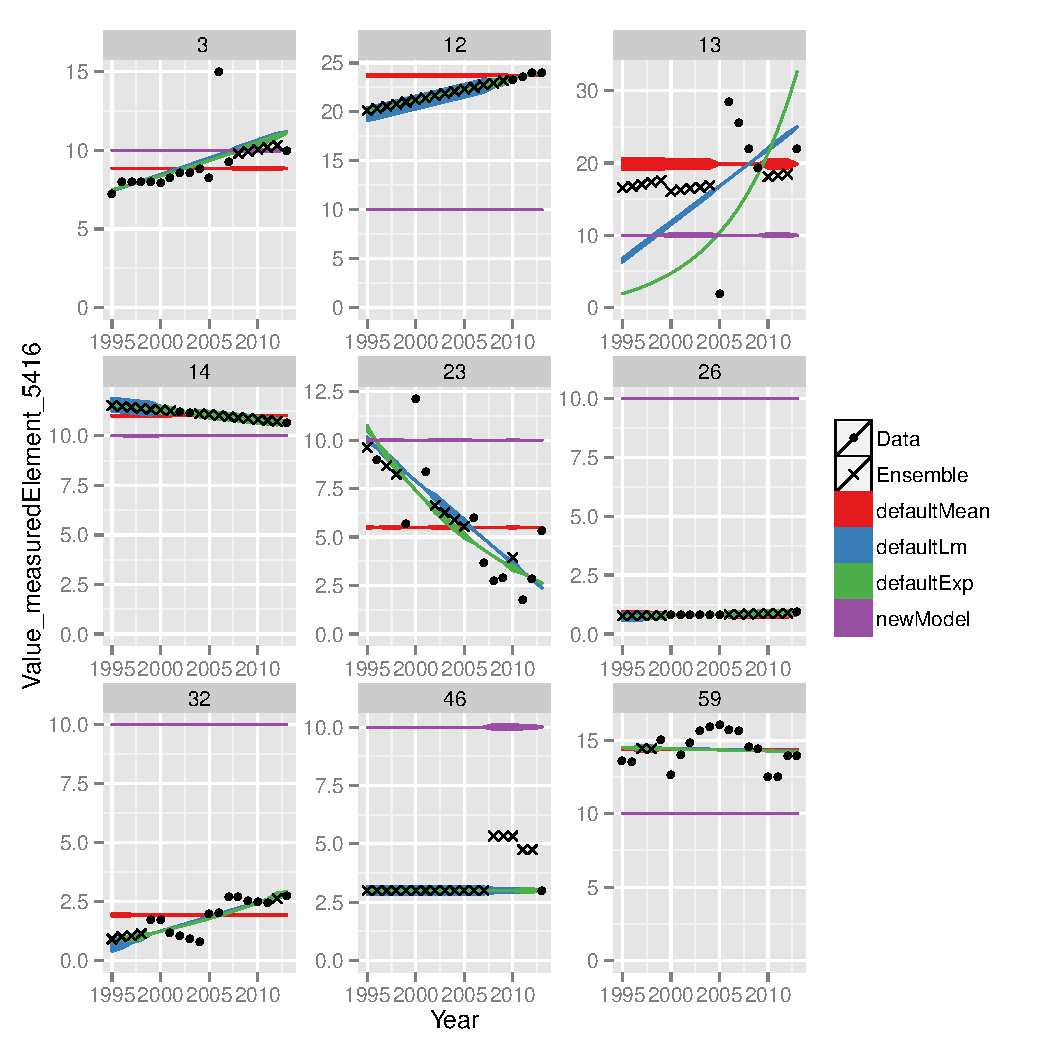
\includegraphics[width=\maxwidth]{figure/impute-yield-1} 

}



\end{knitrout}

Before discussing the output, first note that the newImputationColumn parameter
was updated in the imputationParams object.  This parameter allows you to store
the imputations from the model in three new columns (value, observation flag,
and method flag).  This allows you to examine several different ensembles and
compare their performances.  The default value of
imputationParams\$newImputationColumn is just an empty string, and in this case
the algorithm will place the imputations into the processed data.table.

The graphs contain a lot of information.  First, the dots represent observed
values, and the crosses represent the imputations.  The different colored lines
show the different fits, and the thickness of the line is proportional to the
weight it received in the ensemble.  Of course, if the data point is an
observation then no imputation is done, so all lines have the same thickness
there.  Also, the computed weights will be constant for all imputed values with
one exception: models that are not allowed to extrapolate may have positive
weights for some imputations and 0 for others.  Moreover, if an observation
is outside the extrapolation range of a model, then the weight of all other
models will need to be rescaled so all values add to 1.

We see that the purple line (the model corresponding to our naive model which
always estimates the value 10) rarely gets any weight.  This makes sense, as
it's not a very good model.  However, in some particular cases (i.e.
geographicAreaM49 = 13), no models do very well.  The mean model thus gets most
of the weight, but our naive model also gets a little weight.  You can also see
how it only has weight up to 5 observations outside of the range of the data;
this is because we gave the model an extrapolation range of 5.

Now, suppose we wanted to remove the naive model which always predicts 10.  We
can do that and re-examine what our ensemble looks like:

\begin{knitrout}
\definecolor{shadecolor}{rgb}{0.969, 0.969, 0.969}\color{fgcolor}\begin{kframe}
\begin{alltt}
\hlstd{imputationParams}\hlopt{$}\hlstd{ensembleModels} \hlkwb{=} \hlstd{imputationParams}\hlopt{$}\hlstd{ensembleModels[}\hlopt{-}\hlnum{4}\hlstd{]}
\hlkwd{names}\hlstd{(imputationParams}\hlopt{$}\hlstd{ensembleModels)}
\end{alltt}
\begin{verbatim}
## [1] "defaultMean" "defaultLm"   "defaultExp"
\end{verbatim}
\begin{alltt}
\hlkwd{imputeVariable}\hlstd{(}\hlkwc{data} \hlstd{= okraProcessed,} \hlkwc{imputationParameters} \hlstd{= imputationParams)}
\end{alltt}
\end{kframe}

{\centering 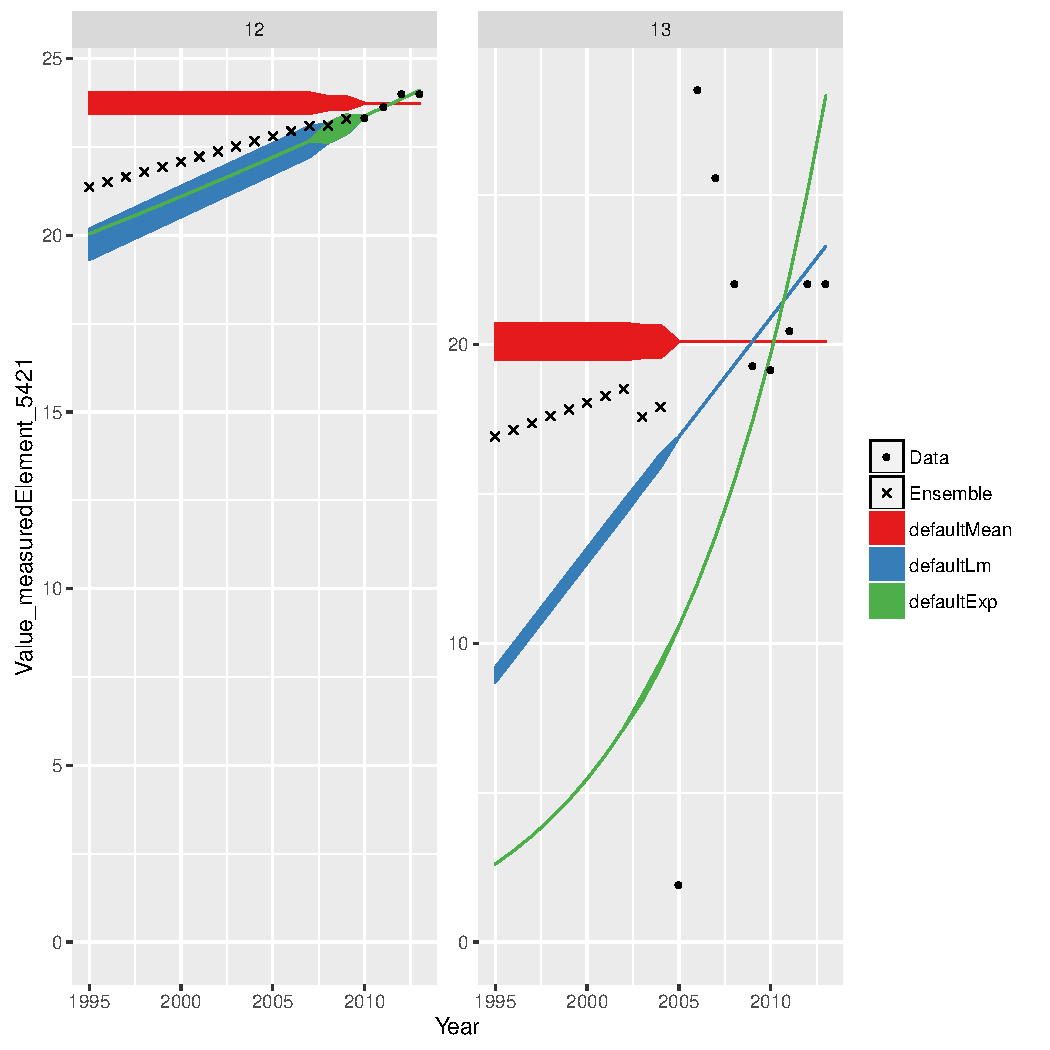
\includegraphics[width=\maxwidth]{figure/unnamed-chunk-2-1} 

}



\end{knitrout}

If we're happy with this model, we can assign these imputed values back to the
original variable:

\begin{knitrout}
\definecolor{shadecolor}{rgb}{0.969, 0.969, 0.969}\color{fgcolor}\begin{kframe}
\begin{alltt}
\hlstd{imputationParams}\hlopt{$}\hlstd{newImputationColumn} \hlkwb{=} \hlstr{""}
\hlkwd{imputeVariable}\hlstd{(}\hlkwc{data} \hlstd{= okraProcessed,} \hlkwc{imputationParameters} \hlstd{= imputationParams)}
\hlkwd{invisible}\hlstd{(okraProcessed[,} \hlkwd{c}\hlstd{(}\hlstr{"Value_test"}\hlstd{,} \hlstr{"flagObservationStatus_test"}\hlstd{,}
                  \hlstr{"flagMethod_test"}\hlstd{)} \hlkwb{:=} \hlkwa{NULL}\hlstd{])}
\end{alltt}
\end{kframe}

{\centering 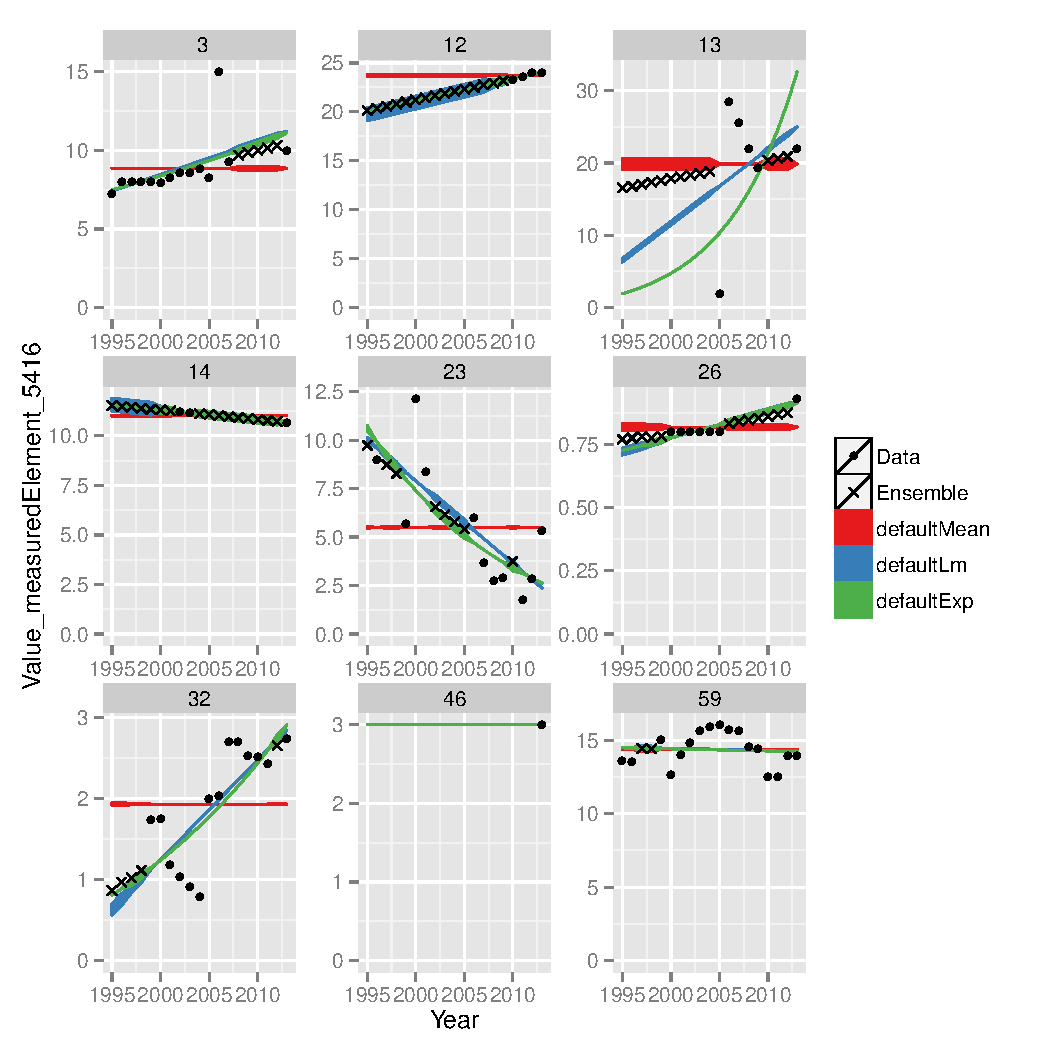
\includegraphics[width=\maxwidth]{figure/unnamed-chunk-3-1} 

}



\end{knitrout}

If we now try to impute again, we see that imputation fails because we have no
missing observations.  Well, to be more accurate, we have missing observations
in one country with only one valid observation.  This country was not
possible to impute because no leave-one-out cross-validation error can be
calculated with a single observation and thus no ensemble weights can be
choosen.

\begin{knitrout}
\definecolor{shadecolor}{rgb}{0.969, 0.969, 0.969}\color{fgcolor}\begin{kframe}
\begin{alltt}
\hlkwd{imputeVariable}\hlstd{(}\hlkwc{data} \hlstd{= okraProcessed,} \hlkwc{imputationParameters} \hlstd{= imputationParams)}
\end{alltt}
\end{kframe}
\end{knitrout}

After the imputation of yield, we proceed to impute the production.  The
function \code{imputeVariable} is used again, but we first need to impute
by ``balancing,'' i.e. updating missing values of production when yield and
area harvested both exist.  This is because we have the relationship:
$$Y = P / A$$
where $Y$ is yield, $P$ is production, and $A$ is the area harvested.
If no value for area harvested is available, then the function proceeds to
impute the remaining production values with ensemble learning.  This balancing
is handled in the faoswsProduction package (which depends on this imputation
package).  To avoid dealing with strange dependency issues, we'll simply ignore
this relationship here.

\begin{knitrout}
\definecolor{shadecolor}{rgb}{0.969, 0.969, 0.969}\color{fgcolor}\begin{kframe}
\begin{alltt}
\hlstd{imputationParams} \hlkwb{=} \hlkwd{defaultImputationParameters}\hlstd{(}\hlstr{"production"}\hlstd{)}
\hlstd{imputationParams}\hlopt{$}\hlstd{ensembleModels} \hlkwb{=}
    \hlstd{imputationParams}\hlopt{$}\hlstd{ensembleModels[}\hlnum{5}\hlopt{:}\hlnum{9}\hlstd{]}
\hlkwd{names}\hlstd{(imputationParams}\hlopt{$}\hlstd{ensembleModels)}
\end{alltt}
\begin{verbatim}
## [1] "defaultLoess"  "defaultSpline" "defaultArima"  "defaultMars"  
## [5] "defaultNaive"
\end{verbatim}
\begin{alltt}
\hlkwd{imputeVariable}\hlstd{(}\hlkwc{data} \hlstd{= okraProcessed,}
               \hlkwc{imputationParameters} \hlstd{= imputationParams)}
\end{alltt}
\end{kframe}

{\centering 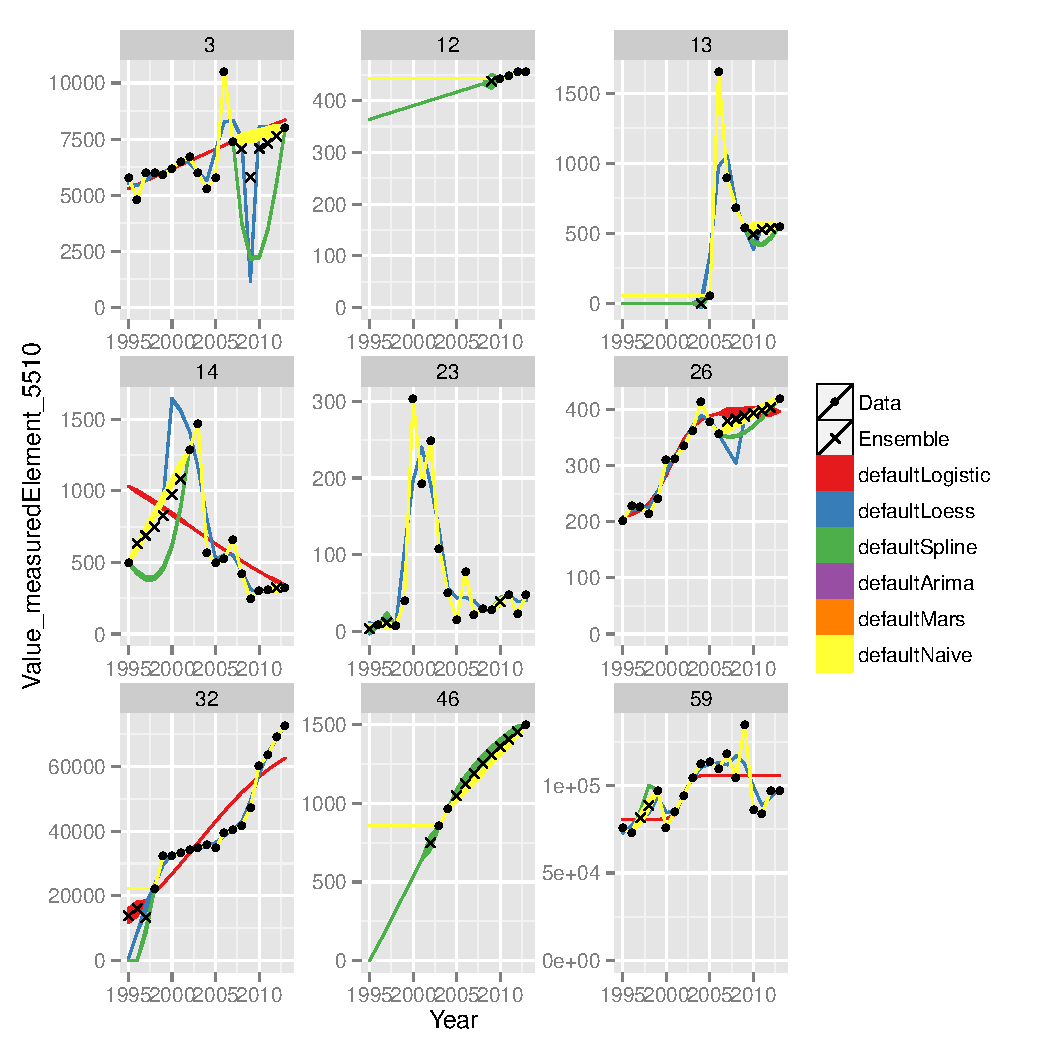
\includegraphics[width=\maxwidth]{figure/impute-production-1} 

}



\end{knitrout}

Note: imputations that are interpolations are always present, but some
extrapolations are not imputed.  The reason for this is that some models are
not reasonable to extrapolate with (such as LOESS, Splines, etc.).  For these
models, an "extrapolation range" is defined, and this value dictates how far
outside the range of the data a particular model is allowed to extrapolate.  In
some cases, no models are valid at a certain range and thus no imputation is
performed.  To avoid these kinds of issues, we recommend including a simple
model that will rarely fail and that can be used to extrapolate (for example,
defaultMean or defaultLm).  Such models will ensure that most values are
imputed.  In our case, the extrapolation ranges are:

\begin{knitrout}
\definecolor{shadecolor}{rgb}{0.969, 0.969, 0.969}\color{fgcolor}\begin{kframe}
\begin{alltt}
\hlkwa{for}\hlstd{(model} \hlkwa{in} \hlstd{imputationParams}\hlopt{$}\hlstd{ensembleModels)}
    \hlkwd{print}\hlstd{(model}\hlopt{@}\hlkwc{extrapolationRange}\hlstd{)}
\end{alltt}
\begin{verbatim}
## [1] 1
## [1] 1
## [1] Inf
## [1] Inf
## [1] 0
\end{verbatim}
\end{kframe}
\end{knitrout}

Thus, the Logistic, Arima, and Mars models are the only models that are allowed
to extrapolate more than one observation away from the data.  For most of the
examples provided here, those three models all failed to fit to the data, and
so imputations were not available.

%' COMMENT BELOW OUT!  DOESN'T WORK WITHOUT faoswsProduction!!!
%'
%' Finally, we can balance the area harvested after both production and
%' yield have been imputed.
%'
%' <<balance-area-harvested>>=
%' balanceAreaHarvested(data = okraProcessed,
%'                      processingParameters = processingParams)
%' @
%'
%'
%' The full procedure outlined in this section can be performed by a
%' single function \code{imputeProductionDomain}.  You will need to specify three
%' parameter lists: the processing parameters (1) and the imputation parameters
%' for both yield and production (2).
%'
%'
%' <<one-step-imputation>>=
%' yieldParams = defaultImputationParameters(5421)
%' yieldParams$ensembleModels = yieldParams$ensembleModels[1:3]
%' productionParams = defaultImputationParameters("production")
%' productionParams$ensembleModels = productionParams$ensembleModels[1:3]
%' okraProcessed = okra[geographicAreaM49 <= 55, ]
%' system.time(
%'     {
%'         imputeProductionDomain(data = okraProcessed,
%'                                processingParameters = processingParams,
%'                                yieldImputationParameters = yieldParams,
%'                                productionImputationParameters =
%'                                    productionParams)
%'     })
%' @


\section{Ensemble model}
Here we provide some details of how to implement user specific
ensemble models.\\

First of all, the component models need to take a vector of values and
return the fitted values. If the model failed, then a vector of NAs equal to
the length of the input should be returned.\\

Shown below is the default linear regression model in the package.  It is the
analyst's job to ensure the component models return sensible values. For
example, negative values are nonsensical for production, and in the current
implementation negative values are replaced with zero.

\begin{knitrout}
\definecolor{shadecolor}{rgb}{0.969, 0.969, 0.969}\color{fgcolor}\begin{kframe}
\begin{alltt}
\hlstd{defaultLm}
\end{alltt}
\begin{verbatim}
## function (x) 
## {
##     stopifnot(is.numeric(x))
##     stopifnot(length(x) > 1)
##     time = 1:length(x)
##     if (all(is.na(x))) 
##         return(as.numeric(rep(NA_real_, length(x))))
##     lmFit = predict(lm(formula = x ~ time), newdata = data.frame(time = time))
##     lmFit[lmFit < 0] = 0
##     lmFit
## }
## <environment: namespace:faoswsImputation>
\end{verbatim}
\end{kframe}
\end{knitrout}

Now, to create an \code{ensembleModel} object, two other pieces of information
must be provided: the extrapolation range of the model (i.e. how many years
it can extrapolate outside the support of the data) and the ``level'' of the
model (see the class documentation):

\begin{knitrout}
\definecolor{shadecolor}{rgb}{0.969, 0.969, 0.969}\color{fgcolor}\begin{kframe}
\begin{alltt}
\hlstd{mod} \hlkwb{=} \hlkwd{ensembleModel}\hlstd{(}\hlkwc{model} \hlstd{= defaultLm,} \hlkwc{extrapolationRange} \hlstd{=} \hlnum{Inf}\hlstd{,}
                    \hlkwc{level} \hlstd{=} \hlstr{"local"}\hlstd{)}
\hlkwd{is}\hlstd{(mod)}
\end{alltt}
\begin{verbatim}
## [1] "ensembleModel"
\end{verbatim}
\end{kframe}
\end{knitrout}

Now, \code{mod} is an object of type ensembleModel.  We can construct a list of
several of these models, but there are also some default models implemented.
Calling allDefaultModels() returns a list of all of these models.

\begin{knitrout}
\definecolor{shadecolor}{rgb}{0.969, 0.969, 0.969}\color{fgcolor}\begin{kframe}
\begin{alltt}
\hlkwd{names}\hlstd{(}\hlkwd{allDefaultModels}\hlstd{())}
\end{alltt}
\begin{verbatim}
##  [1] "defaultMean"       "defaultLm"         "defaultExp"       
##  [4] "defaultLogistic"   "defaultLoess"      "defaultSpline"    
##  [7] "defaultArima"      "defaultMars"       "defaultNaive"     
## [10] "defaultMixedModel"
\end{verbatim}
\begin{alltt}
\hlkwd{sapply}\hlstd{(}\hlkwd{allDefaultModels}\hlstd{(), is)}
\end{alltt}
\begin{verbatim}
##       defaultMean         defaultLm        defaultExp   defaultLogistic 
##   "ensembleModel"   "ensembleModel"   "ensembleModel"   "ensembleModel" 
##      defaultLoess     defaultSpline      defaultArima       defaultMars 
##   "ensembleModel"   "ensembleModel"   "ensembleModel"   "ensembleModel" 
##      defaultNaive defaultMixedModel 
##   "ensembleModel"   "ensembleModel"
\end{verbatim}
\end{kframe}
\end{knitrout}

Here we take the Okra production value of Bahrain as an
illustration. After the component models have been designed and
inserted into a list, we can compute the fits and weights then
combine it to form the ensemble with the following functions.

First, we have to make sure we've correctly labeled any missing values as NA
and not 0:

\begin{knitrout}
\definecolor{shadecolor}{rgb}{0.969, 0.969, 0.969}\color{fgcolor}\begin{kframe}
\begin{alltt}
\hlstd{bahrainExample} \hlkwb{=} \hlstd{okra[areaName} \hlopt{==} \hlstr{"Bahrain"}\hlstd{, ]}
\hlstd{bahrainExample[}\hlnum{1}\hlopt{:}\hlnum{4}\hlstd{,} \hlkwd{.}\hlstd{(areaName, timePointYears,}
                      \hlkwc{production} \hlstd{= Value_measuredElement_5510,}
                      \hlkwc{productionFlag} \hlstd{=}
                          \hlstd{flagObservationStatus_measuredElement_5510)]}
\end{alltt}
\begin{verbatim}
##    areaName timePointYears production productionFlag
## 1:  Bahrain           1995          0              M
## 2:  Bahrain           1996          0              M
## 3:  Bahrain           1997          0              M
## 4:  Bahrain           1998          0              M
\end{verbatim}
\begin{alltt}
\hlstd{bahrainExample} \hlkwb{=}
    \hlkwd{remove0M}\hlstd{(}\hlkwc{data} \hlstd{= bahrainExample,}
             \hlkwc{valueVars} \hlstd{=} \hlstr{"Value_measuredElement_5510"}\hlstd{,}
             \hlkwc{flag} \hlstd{=} \hlstr{"flagObservationStatus_measuredElement_5510"}\hlstd{)}
\hlstd{bahrainExample[}\hlnum{1}\hlopt{:}\hlnum{4}\hlstd{,} \hlkwd{.}\hlstd{(areaName, timePointYears,}
                      \hlkwc{production} \hlstd{= Value_measuredElement_5510,}
                      \hlkwc{productionFlag} \hlstd{=}
                          \hlstd{flagObservationStatus_measuredElement_5510)]}
\end{alltt}
\begin{verbatim}
##    areaName timePointYears production productionFlag
## 1:  Bahrain           1995         NA              M
## 2:  Bahrain           1996         NA              M
## 3:  Bahrain           1997         NA              M
## 4:  Bahrain           1998         NA              M
\end{verbatim}
\end{kframe}
\end{knitrout}

Next, we compute the model fits.  We'll print the first three fits:

\begin{knitrout}
\definecolor{shadecolor}{rgb}{0.969, 0.969, 0.969}\color{fgcolor}\begin{kframe}
\begin{alltt}
\hlcom{## Compute fit for all component models}
\hlstd{imputationParameters} \hlkwb{=} \hlkwd{defaultImputationParameters}\hlstd{(}\hlstr{"production"}\hlstd{)}
\hlstd{modelFits} \hlkwb{=} \hlkwd{computeEnsembleFit}\hlstd{(}\hlkwc{data} \hlstd{= bahrainExample,}
                               \hlkwc{imputationParameters} \hlstd{= imputationParameters)}
\hlstd{modelFits[}\hlnum{1}\hlopt{:}\hlnum{3}\hlstd{]}
\end{alltt}
\begin{verbatim}
## $defaultMean
##  [1] 659.3333 659.3333 659.3333 659.3333 659.3333 659.3333 659.3333 659.3333
##  [9] 659.3333 659.3333 659.3333 659.3333 659.3333 659.3333 659.3333 659.3333
## [17] 659.3333 659.3333 659.3333
## 
## $defaultLm
##  [1] 1191.5667 1153.5500 1115.5333 1077.5167 1039.5000 1001.4833  963.4667
##  [8]  925.4500  887.4333  849.4167  811.4000  773.3833  735.3667  697.3500
## [15]  659.3333  621.3167  583.3000  545.2833  507.2667
## 
## $defaultExp
##  [1] 181.4353 195.3650 210.3582 226.4962 243.8665 262.5630 282.6871 304.3477
##  [9] 327.6622 352.7568 379.7676 408.8407 440.1336 473.8159 510.0700 549.0922
## [17] 591.0939 636.3026 684.9631
\end{verbatim}
\begin{alltt}
\hlkwd{length}\hlstd{(modelFits)}
\end{alltt}
\begin{verbatim}
## [1] 10
\end{verbatim}
\end{kframe}
\end{knitrout}

To compute weights, we need to use cross-validation.  Each observation is
assigned a cross-validation group.  To compute the error of a particular model,
we estimate the observed values in group i with all values not in group i.
This allows us to measure how well a model predicts the data, and can help
prevent overfitting.  The model weights are then computed.  Note the NA's;
these exist when observations are real and values are not being imputed.

\begin{knitrout}
\definecolor{shadecolor}{rgb}{0.969, 0.969, 0.969}\color{fgcolor}\begin{kframe}
\begin{alltt}
\hlcom{## Calculate the weight for each component model}
\hlstd{cvGroup} \hlkwb{=} \hlkwd{makeCvGroup}\hlstd{(}\hlkwc{data} \hlstd{= bahrainExample,}
                      \hlkwc{imputationParameters} \hlstd{= imputationParameters)}
\hlstd{cvGroup}
\end{alltt}
\begin{verbatim}
##  [1] NA NA NA NA NA NA NA NA NA NA  3  8 10  4  5  6  1  7  2
\end{verbatim}
\begin{alltt}
\hlstd{modelStats} \hlkwb{=} \hlkwd{computeEnsembleWeight}\hlstd{(}\hlkwc{data} \hlstd{= bahrainExample,}
                                   \hlkwc{cvGroup} \hlstd{= cvGroup,}
                                   \hlkwc{fits} \hlstd{= modelFits,}
                                   \hlkwc{method} \hlstd{=} \hlstr{"inverse"}\hlstd{,}
                                   \hlkwc{imputationParameters} \hlstd{=}
                                       \hlstd{imputationParameters)}
\hlstd{modelWeights} \hlkwb{=} \hlstd{modelStats[[}\hlnum{1}\hlstd{]]}
\hlstd{modelWeights[,} \hlkwd{c}\hlstd{(}\hlstr{"defaultArima"}\hlstd{,} \hlstr{"defaultExp"}\hlstd{,} \hlstr{"defaultLm"}\hlstd{)]}
\end{alltt}
\begin{verbatim}
## [1] "defaultArima" "defaultExp"   "defaultLm"
\end{verbatim}
\begin{alltt}
\hlkwd{dim}\hlstd{(modelWeights)}
\end{alltt}
\begin{verbatim}
## [1] 19 10
\end{verbatim}
\end{kframe}
\end{knitrout}

Lastly, combine the fits with the estimated weights to produce the final
ensemble, and then plot it!

\begin{knitrout}
\definecolor{shadecolor}{rgb}{0.969, 0.969, 0.969}\color{fgcolor}\begin{kframe}
\begin{alltt}
\hlcom{## Combine the models to obtain the ensemble}
\hlstd{ensemble} \hlkwb{=} \hlstd{bahrainExample[, Value_measuredElement_5510]}
\hlstd{modelErrors} \hlkwb{=} \hlstd{modelStats[[}\hlnum{2}\hlstd{]]}
\hlstd{imputationFit} \hlkwb{=} \hlkwd{computeEnsemble}\hlstd{(modelFits, modelWeights, modelErrors)}
\hlstd{ensemble[}\hlkwd{is.na}\hlstd{(ensemble)]} \hlkwb{=} \hlstd{imputationFit[}\hlkwd{is.na}\hlstd{(ensemble), fit]}
\hlkwd{plotEnsemble}\hlstd{(}\hlkwc{data} \hlstd{= bahrainExample,} \hlkwc{modelFits} \hlstd{= modelFits,}
             \hlkwc{modelWeights} \hlstd{= modelWeights,} \hlkwc{ensemble} \hlstd{= ensemble,}
             \hlkwc{imputationParameters} \hlstd{= imputationParameters)}
\end{alltt}
\begin{verbatim}
## NULL
\end{verbatim}
\end{kframe}

{\centering 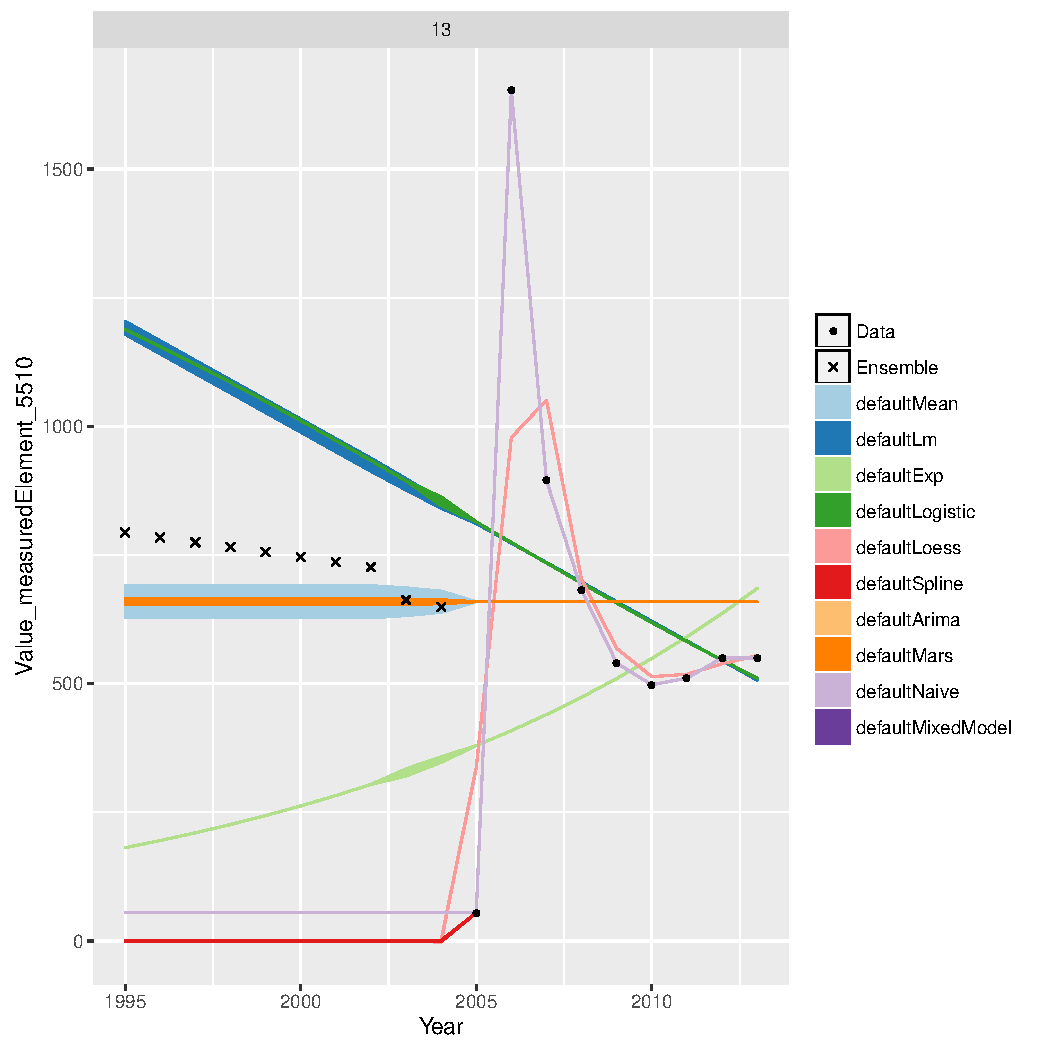
\includegraphics[width=\maxwidth]{figure/unnamed-chunk-8-1} 

}



\end{knitrout}

A one-step wrapper function is also available.  There are also many other
options you can specify when constructing an ensemble, such as the maximum
weight that may be given to a model or a custom error function for choosing
weights.  See defaultImputationParameters for a description of all the options.

\begin{knitrout}
\definecolor{shadecolor}{rgb}{0.969, 0.969, 0.969}\color{fgcolor}\begin{kframe}
\begin{alltt}
\hlstd{bahamasExample} \hlkwb{=} \hlstd{okra[areaName} \hlopt{==} \hlstr{"Bahamas"}\hlstd{, ]}
\hlstd{bahamasExample} \hlkwb{=}
    \hlkwd{remove0M}\hlstd{(}\hlkwc{data} \hlstd{= bahamasExample,}
             \hlkwc{valueVars} \hlstd{=} \hlstr{"Value_measuredElement_5510"}\hlstd{,}
             \hlkwc{flag} \hlstd{=} \hlstr{"flagObservationStatus_measuredElement_5510"}\hlstd{)}
\hlstd{ensembleFit} \hlkwb{=} \hlkwd{ensembleImpute}\hlstd{(}\hlkwc{data} \hlstd{= bahamasExample,}
                             \hlkwc{imputationParameters} \hlstd{= imputationParameters)}
\end{alltt}
\end{kframe}

{\centering 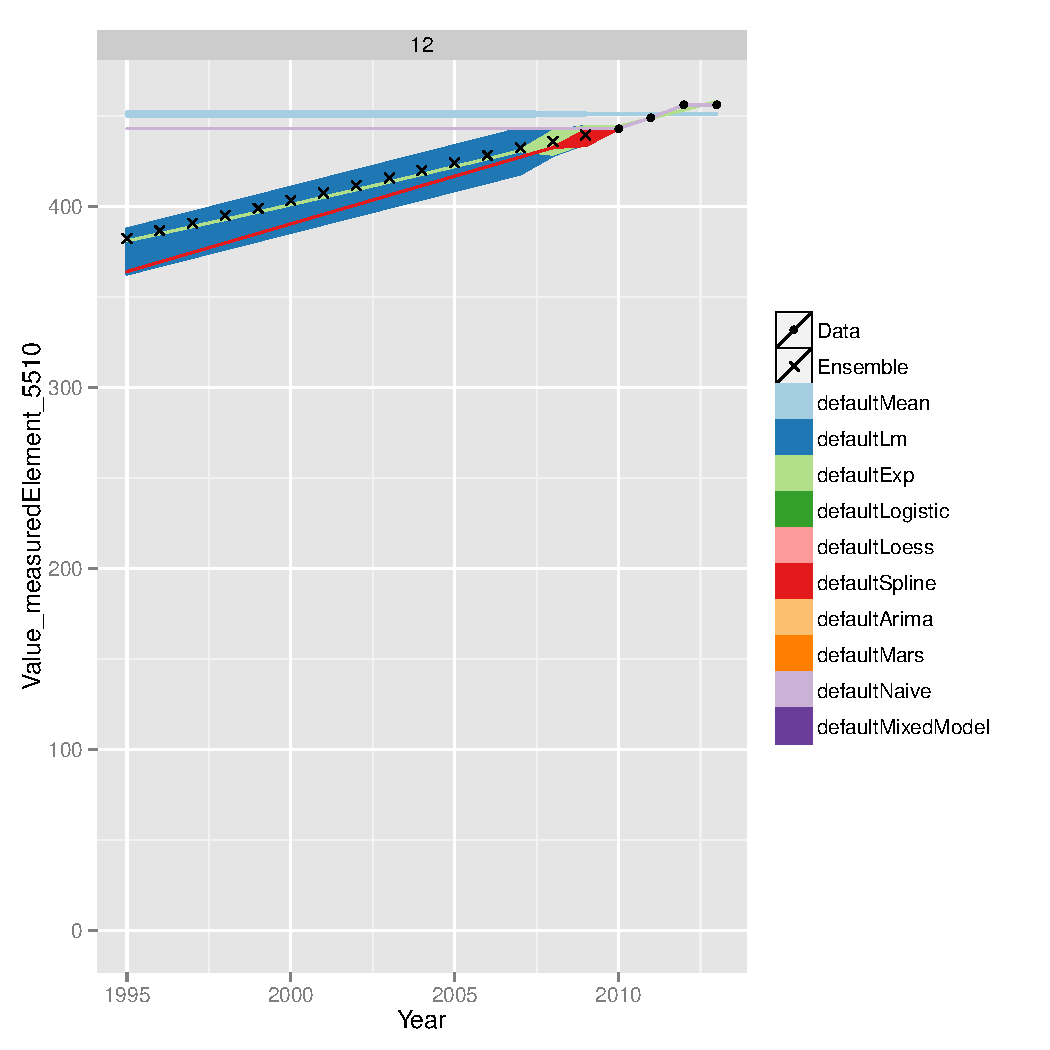
\includegraphics[width=\maxwidth]{figure/ensemble-imputation-1} 

}



\end{knitrout}

\section{Models for Ensembling}

This package implements many complex models that may not be familiar to the
user, and so this section goes through the models and describes
how the algorithm works as well as gives an example of the usage of that model.
The order of this section is alphabetical, not by complexity.  Let's first set
up a dataset to use for this example, and we'll set

\begin{knitrout}
\definecolor{shadecolor}{rgb}{0.969, 0.969, 0.969}\color{fgcolor}\begin{kframe}
\begin{alltt}
\hlstd{exampleData} \hlkwb{=} \hlstd{okra[geographicAreaM49} \hlopt{<} \hlnum{60}\hlstd{, ]}
\hlstd{imputationParameters} \hlkwb{=} \hlkwd{defaultImputationParameters}\hlstd{(}\hlnum{5421}\hlstd{)}
\hlstd{imputationParameters}\hlopt{$}\hlstd{newImputationColumn} \hlkwb{=} \hlstr{"test"}
\hlkwd{invisible}\hlstd{(exampleData[timePointYears} \hlopt \hlnum{2005}\hlopt{:}\hlnum{2007} \hlopt{&}
                          \hlstd{geographicAreaM49} \hlopt{==} \hlstr{"91"}\hlstd{,}
                      \hlkwd{c}\hlstd{(}\hlstr{"Value_measuredElement_5421"}\hlstd{,}
                        \hlstr{"flagObservationStatus_measuredElement_5421"}\hlstd{)} \hlkwb{:=}
                          \hlkwd{list}\hlstd{(}\hlnum{NA}\hlstd{,} \hlstr{"M"}\hlstd{)])}
\end{alltt}
\end{kframe}
\end{knitrout}

\subsection{defaultArima}

The defaultArima model first fits an AutoRegressive, Integrated Moving Average
(ARIMA) model to the time series provided, and it attempts to find the best
model using the auto.arima function from the \pkg{forecast} package.  If such a
model is found, that model is used (along with KalmanSmooth) to generate
new smoothed estimates of the time series.

\begin{knitrout}
\definecolor{shadecolor}{rgb}{0.969, 0.969, 0.969}\color{fgcolor}\begin{kframe}
\begin{alltt}
\hlstd{model} \hlkwb{=} \hlkwd{ensembleModel}\hlstd{(}\hlkwc{model} \hlstd{= defaultArima,} \hlkwc{extrapolationRange} \hlstd{=} \hlnum{Inf}\hlstd{,}
                      \hlkwc{level} \hlstd{=} \hlstr{"local"}\hlstd{)}
\hlstd{imputationParameters}\hlopt{$}\hlstd{ensembleModels} \hlkwb{=} \hlkwd{list}\hlstd{(model)}
\hlkwd{imputeVariable}\hlstd{(}\hlkwc{data} \hlstd{= exampleData,} \hlkwc{imputationParameters} \hlstd{= imputationParameters)}
\end{alltt}
\end{kframe}

{\centering 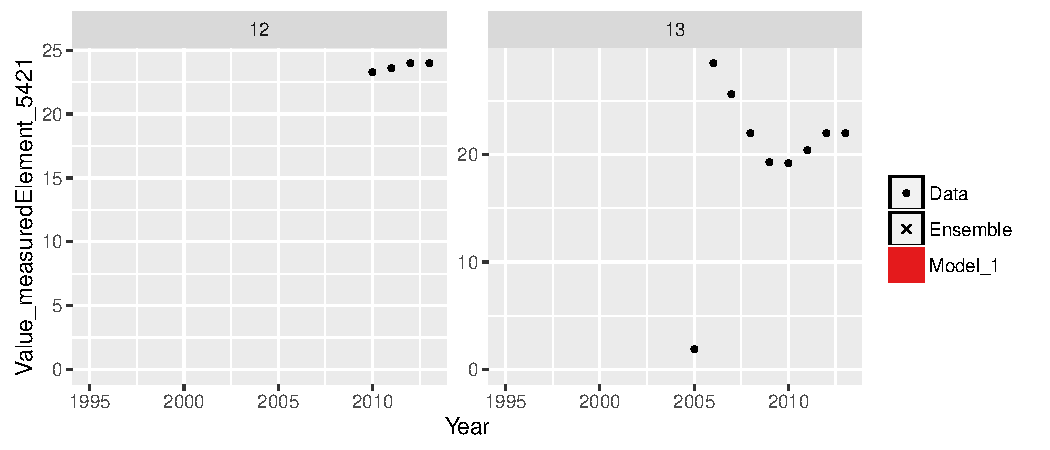
\includegraphics[width=\maxwidth]{figure/unnamed-chunk-9-1} 

}



\end{knitrout}

%' This model often fails, on FAO time-series, and in such cases it is not used in
%' the final ensemble.  Below is an example of when it succeeds, though:
%'
%' <<fig.height=3>>=
%' x = arima.sim(n = 100, model = list(ar = .9))
%' qplot(1:100, x) + geom_line(aes(y = defaultArima(x)))
%' @
%'
%' This example shows one of the common features of the default models: they often
%' set negative values to 0 (as this is the most reasonable thing to do with most
%' of the FAO data).  However, there may be variables where negative values are
%' reasonable, and in such cases an adjusted model should be used.

\subsection{defaultExp}

This algorithm fits the following model: $\log(Y+1) = \beta_0 + \beta_1 t$
where $Y$ is the dependent variable (i.e. production, seed rates, etc) $t$
is time, and $\beta_0, \beta_1$ are the estimated coefficients.  This model is
equivalent to $Y + 1 = e^{\beta_0 + \beta_1 t}$, hence the name exponential.
The 1 in the formula ensures that $\log(Y+1)$ always exists (assuming
$Y \geq 0$).

\begin{knitrout}
\definecolor{shadecolor}{rgb}{0.969, 0.969, 0.969}\color{fgcolor}\begin{kframe}
\begin{alltt}
\hlstd{model} \hlkwb{=} \hlkwd{ensembleModel}\hlstd{(}\hlkwc{model} \hlstd{= defaultExp,} \hlkwc{extrapolationRange} \hlstd{=} \hlnum{1}\hlstd{,}
                      \hlkwc{level} \hlstd{=} \hlstr{"local"}\hlstd{)}
\hlstd{imputationParameters}\hlopt{$}\hlstd{ensembleModels} \hlkwb{=} \hlkwd{list}\hlstd{(model)}
\hlkwd{imputeVariable}\hlstd{(}\hlkwc{data} \hlstd{= exampleData,} \hlkwc{imputationParameters} \hlstd{= imputationParameters)}
\end{alltt}
\end{kframe}

{\centering 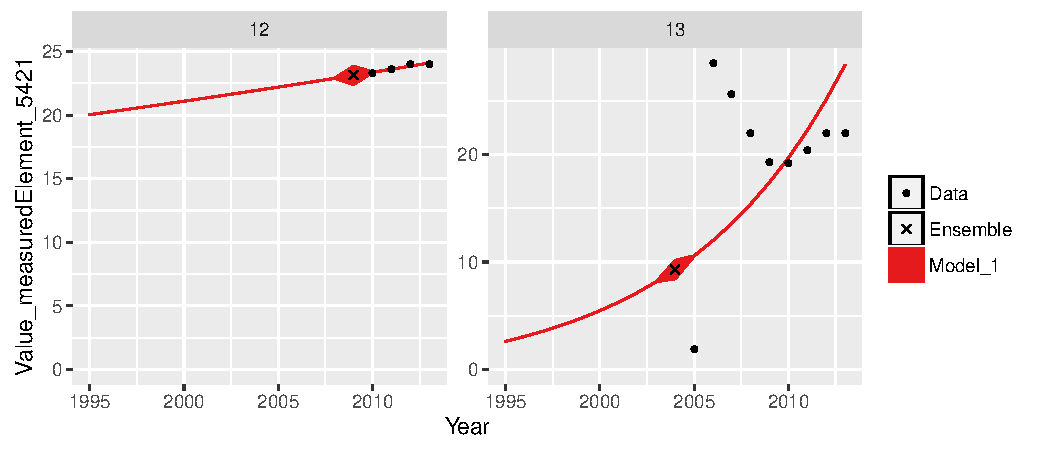
\includegraphics[width=\maxwidth]{figure/unnamed-chunk-10-1} 

}



\end{knitrout}

\subsection{defaultGlobalMean}

This model is quite simple: it computes the mean from all available
observations and uses that value to impute any missing values.  This model is
not recommended for most domains; however, it may perform reasonably well when
imputing rates or proportions, as the average may not vary drastically from
country to country.  A variable like production is very different, values can
vary drastically in scale and so a global mean is not appropriate.

\begin{knitrout}
\definecolor{shadecolor}{rgb}{0.969, 0.969, 0.969}\color{fgcolor}\begin{kframe}
\begin{alltt}
\hlstd{model} \hlkwb{=} \hlkwd{ensembleModel}\hlstd{(}\hlkwc{model} \hlstd{= defaultGlobalMean,} \hlkwc{extrapolationRange} \hlstd{=} \hlnum{Inf}\hlstd{,}
                      \hlkwc{level} \hlstd{=} \hlstr{"global"}\hlstd{)}
\hlstd{imputationParameters}\hlopt{$}\hlstd{ensembleModels} \hlkwb{=} \hlkwd{list}\hlstd{(model)}
\hlkwd{imputeVariable}\hlstd{(}\hlkwc{data} \hlstd{= exampleData,} \hlkwc{imputationParameters} \hlstd{= imputationParameters)}
\end{alltt}
\end{kframe}

{\centering 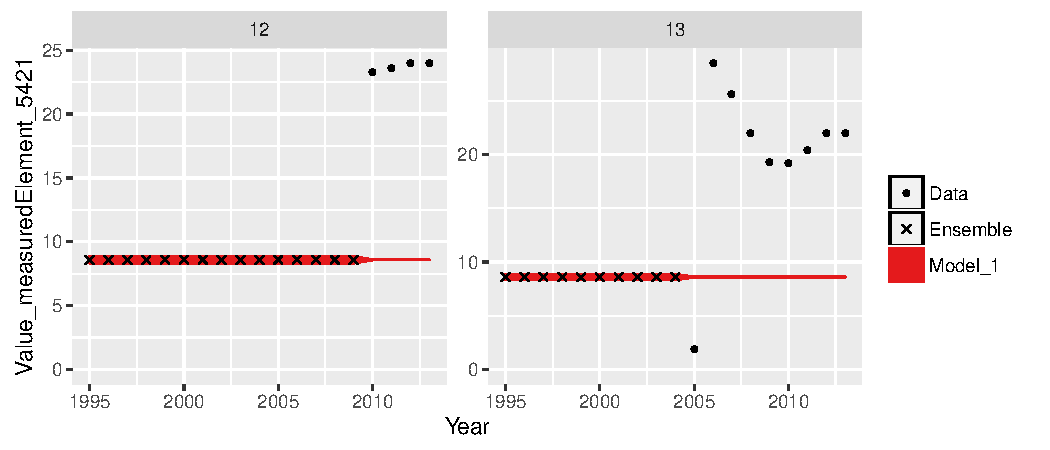
\includegraphics[width=\maxwidth]{figure/unnamed-chunk-11-1} 

}



\end{knitrout}

Note that in the above figure, the imputed values may appear to be different.
However, this is simply due to the different scale in each of the grids; the
imputed value is always about 8.

\subsection{defaultGlobalMedian}

The global median works exactly the same as the global mean, but computes the
median instead of the mean.  Again, this type of model should only be used when
imputing rates or something similar (i.e. no drastic differences in scale
across groups).

\begin{knitrout}
\definecolor{shadecolor}{rgb}{0.969, 0.969, 0.969}\color{fgcolor}\begin{kframe}
\begin{alltt}
\hlstd{model} \hlkwb{=} \hlkwd{ensembleModel}\hlstd{(}\hlkwc{model} \hlstd{= defaultGlobalMedian,} \hlkwc{extrapolationRange} \hlstd{=} \hlnum{Inf}\hlstd{,}
                      \hlkwc{level} \hlstd{=} \hlstr{"global"}\hlstd{)}
\hlstd{imputationParameters}\hlopt{$}\hlstd{ensembleModels} \hlkwb{=} \hlkwd{list}\hlstd{(model)}
\hlkwd{imputeVariable}\hlstd{(}\hlkwc{data} \hlstd{= exampleData,} \hlkwc{imputationParameters} \hlstd{= imputationParameters)}
\end{alltt}
\end{kframe}

{\centering 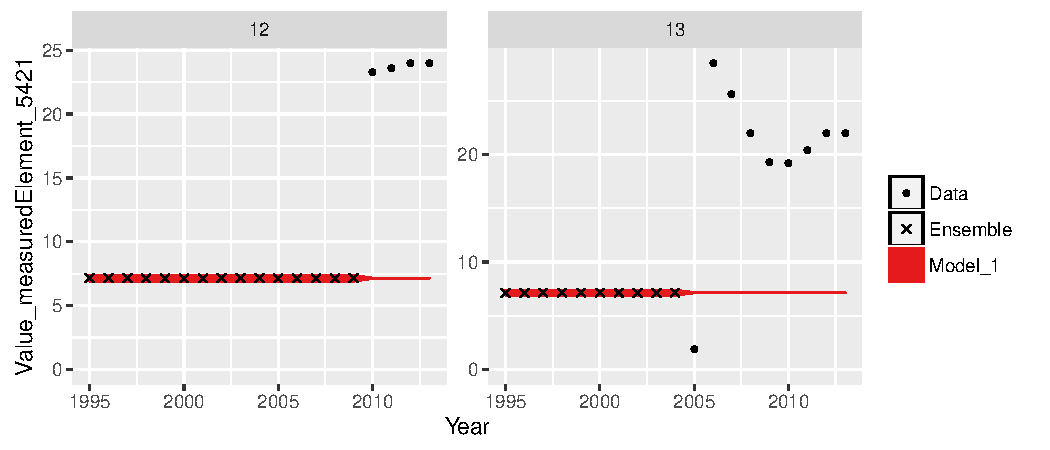
\includegraphics[width=\maxwidth]{figure/unnamed-chunk-12-1} 

}



\end{knitrout}

\subsection{defaultLm}

The defaultLm model uses a simple linear regression model for imputation.  It
fits a model of the form: $Y = \beta_0 + \beta_1 t$, where $Y$ is the value to
impute, $t$ is the time, and $\beta_0, \beta_1$ are estimated coefficients.

\begin{knitrout}
\definecolor{shadecolor}{rgb}{0.969, 0.969, 0.969}\color{fgcolor}\begin{kframe}
\begin{alltt}
\hlstd{model} \hlkwb{=} \hlkwd{ensembleModel}\hlstd{(}\hlkwc{model} \hlstd{= defaultLm,} \hlkwc{extrapolationRange} \hlstd{=} \hlnum{Inf}\hlstd{,}
                      \hlkwc{level} \hlstd{=} \hlstr{"local"}\hlstd{)}
\hlstd{imputationParameters}\hlopt{$}\hlstd{ensembleModels} \hlkwb{=} \hlkwd{list}\hlstd{(model)}
\hlkwd{imputeVariable}\hlstd{(}\hlkwc{data} \hlstd{= exampleData,} \hlkwc{imputationParameters} \hlstd{= imputationParameters)}
\end{alltt}
\end{kframe}

{\centering 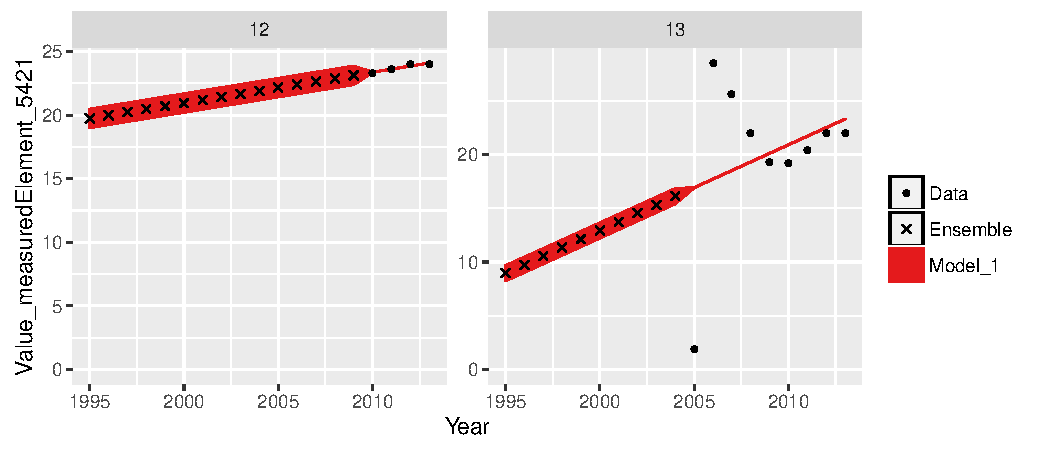
\includegraphics[width=\maxwidth]{figure/unnamed-chunk-13-1} 

}



\end{knitrout}

\subsection{defaultLoess}

The defaultLoess model works by fitting a ``local'' linear regression model at
each point in the model space.  The model is local in the sense that the fit at
time $t$ uses only nearby time points, say $t-k$ to $t+k$.  Furthermore, points
further away from $t$ are given less weight in the regression model.  This type
of model has several tuning parameters such as the size of the neighborhood and
the degree of model to fit (i.e. we could fit local linear models, quadratic,
etc.).  For simplicity, we use a local linear model, and we choose the smallest
span possible to allow for the most flexible model.  Addditionally, the local
nature of the loess model means that it likely will not extrapolate well, so
the recommended extrapolation range is 1.

\begin{knitrout}
\definecolor{shadecolor}{rgb}{0.969, 0.969, 0.969}\color{fgcolor}\begin{kframe}
\begin{alltt}
\hlstd{model} \hlkwb{=} \hlkwd{ensembleModel}\hlstd{(}\hlkwc{model} \hlstd{= defaultLoess,} \hlkwc{extrapolationRange} \hlstd{=} \hlnum{1}\hlstd{,}
                      \hlkwc{level} \hlstd{=} \hlstr{"local"}\hlstd{)}
\hlstd{imputationParameters}\hlopt{$}\hlstd{ensembleModels} \hlkwb{=} \hlkwd{list}\hlstd{(model)}
\hlkwd{imputeVariable}\hlstd{(}\hlkwc{data} \hlstd{= exampleData,} \hlkwc{imputationParameters} \hlstd{= imputationParameters)}
\end{alltt}
\end{kframe}

{\centering 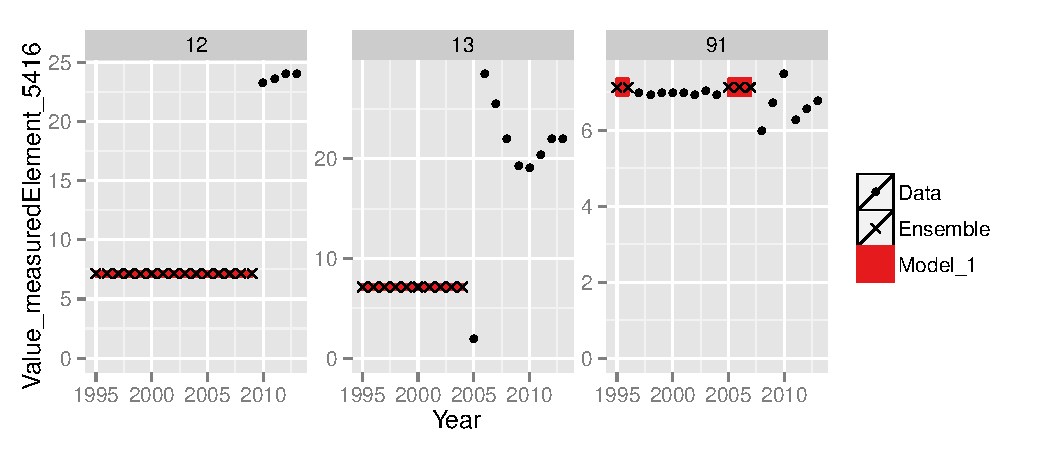
\includegraphics[width=\maxwidth]{figure/unnamed-chunk-14-1} 

}



\end{knitrout}

\subsection{defaultLogistic}

Logistic curves are S-shaped curves of the form
$$f(x) = A + \frac{B}{1 + e^{-C(t-D)}}$$.
These types of functions make sense in scenarios where a variable is increasing
but may have some upper bound (i.e. production may increase greatly as
technology improves, but there is some maximum production level a country can
obtain).  This algorithm attempts to first fit all four parameters above via
numerical least squares.  If that approach fails, $A$ is assumed to be 0 and
numerical least squares are tried again.  If that model also fails, $B$ is
assumed to be the largest value and model fitting proceeds via generalized
least squares.

\begin{knitrout}
\definecolor{shadecolor}{rgb}{0.969, 0.969, 0.969}\color{fgcolor}\begin{kframe}
\begin{alltt}
\hlstd{model} \hlkwb{=} \hlkwd{ensembleModel}\hlstd{(}\hlkwc{model} \hlstd{= defaultLogistic,} \hlkwc{extrapolationRange} \hlstd{=} \hlnum{1}\hlstd{,}
                      \hlkwc{level} \hlstd{=} \hlstr{"local"}\hlstd{)}
\hlstd{imputationParameters}\hlopt{$}\hlstd{ensembleModels} \hlkwb{=} \hlkwd{list}\hlstd{(model)}
\hlkwd{imputeVariable}\hlstd{(}\hlkwc{data} \hlstd{= exampleData,} \hlkwc{imputationParameters} \hlstd{= imputationParameters)}
\end{alltt}
\end{kframe}

{\centering 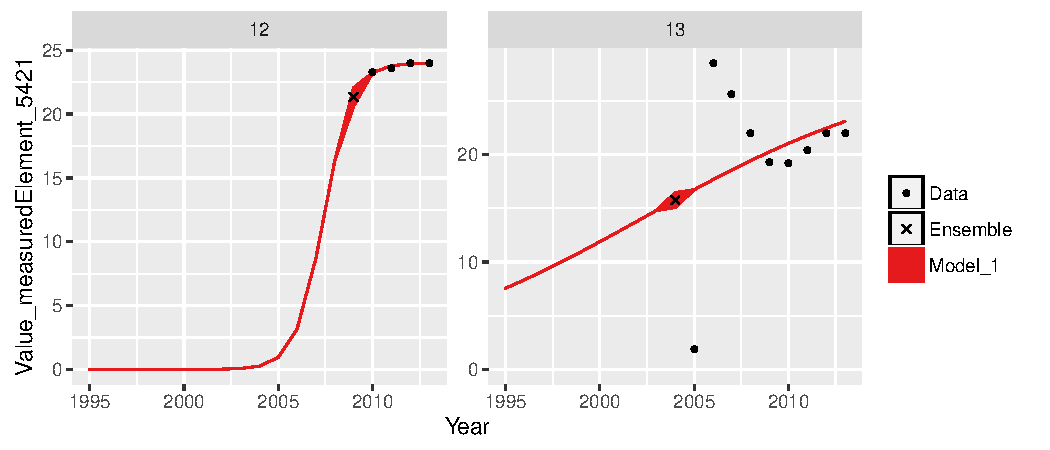
\includegraphics[width=\maxwidth]{figure/unnamed-chunk-15-1} 

}



\end{knitrout}

Note: in the first example, the logistic regression decays rapidly to 0.  This may not be very reasonable, and thus we recommend using a small extrapolation range for this model.

\subsection{defaultMars}

The defaultMars model uses a technique known as Multivariate Adaptive
Regression Splines (MARS).  This algorithm seeks to model the data using
piecewise linear regression splines, and it determines the breakpoints of the
splines using some optimization criterion.  On our sample dataset, we don't see
anything too interesting:

\begin{knitrout}
\definecolor{shadecolor}{rgb}{0.969, 0.969, 0.969}\color{fgcolor}\begin{kframe}
\begin{alltt}
\hlstd{model} \hlkwb{=} \hlkwd{ensembleModel}\hlstd{(}\hlkwc{model} \hlstd{= defaultMars,} \hlkwc{extrapolationRange} \hlstd{=} \hlnum{Inf}\hlstd{,}
                      \hlkwc{level} \hlstd{=} \hlstr{"local"}\hlstd{)}
\hlstd{imputationParameters}\hlopt{$}\hlstd{ensembleModels} \hlkwb{=} \hlkwd{list}\hlstd{(model)}
\hlkwd{imputeVariable}\hlstd{(}\hlkwc{data} \hlstd{= exampleData,} \hlkwc{imputationParameters} \hlstd{= imputationParameters)}
\end{alltt}
\end{kframe}

{\centering 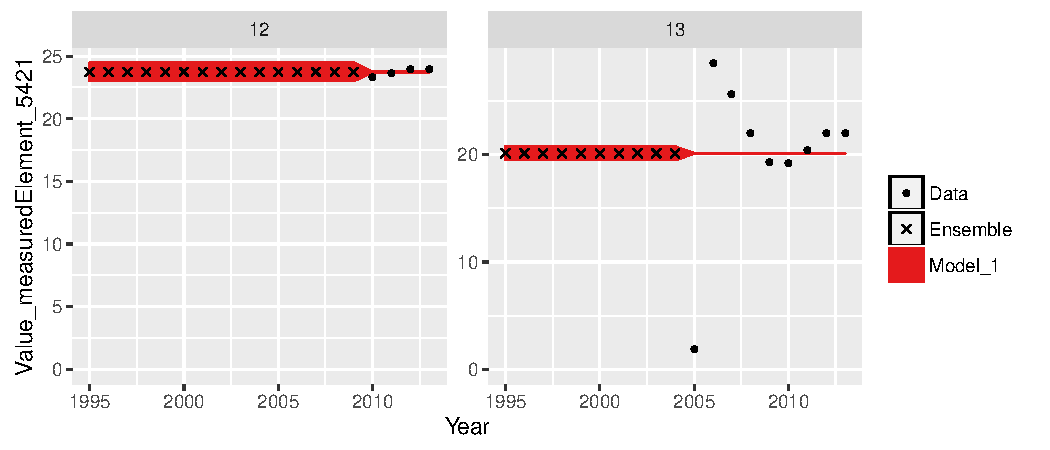
\includegraphics[width=\maxwidth]{figure/unnamed-chunk-16-1} 

}



\end{knitrout}

%' To see how this model works, we can instead look at a little toy example.
%' Suppose that our data is constant for the first 10 observations and then
%' increases linearly for the following 10 observations.  And, suppose that we
%' can't measure our data perfectly, but that we have some observation error.
%' The below R code implements such a model, and shows how the MARS approach will
%' fit that data (MARS is named ``earth'' within R because MARS is a proprietary
%' term).
%'
%' <<fig.height=3>>=
%' smallExample = data.table(x = 1:20, y = c(rep(0, 10), 1:10) +
%'                               rnorm(20, sd = .2))
%' fit = earth::earth(y ~ x, data = smallExample)
%' invisible(smallExample[, earthFit := predict(fit)])
%' ggplot(smallExample, aes(x = x, y = y)) + geom_point() +
%'     geom_line(aes(y = earthFit))
%' @

\subsection{defaultMean}

This model computes a mean on each subset of the data and uses that one value to
impute any missing values.

\begin{knitrout}
\definecolor{shadecolor}{rgb}{0.969, 0.969, 0.969}\color{fgcolor}\begin{kframe}
\begin{alltt}
\hlstd{model} \hlkwb{=} \hlkwd{ensembleModel}\hlstd{(}\hlkwc{model} \hlstd{= defaultMean,} \hlkwc{extrapolationRange} \hlstd{=} \hlnum{Inf}\hlstd{,}
                      \hlkwc{level} \hlstd{=} \hlstr{"local"}\hlstd{)}
\hlstd{imputationParameters}\hlopt{$}\hlstd{ensembleModels} \hlkwb{=} \hlkwd{list}\hlstd{(model)}
\hlkwd{imputeVariable}\hlstd{(}\hlkwc{data} \hlstd{= exampleData,} \hlkwc{imputationParameters} \hlstd{= imputationParameters)}
\end{alltt}
\end{kframe}

{\centering 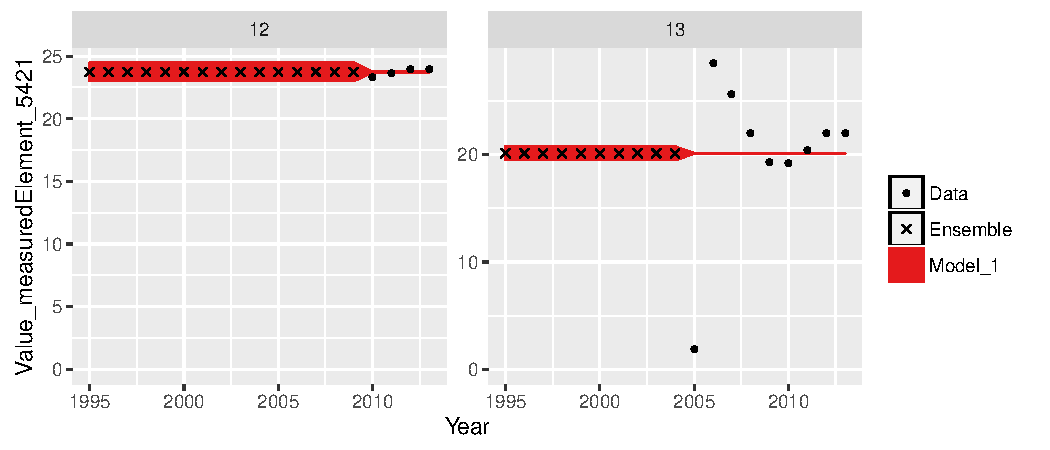
\includegraphics[width=\maxwidth]{figure/unnamed-chunk-17-1} 

}



\end{knitrout}

\subsection{defaultMedian}

This model computes a median on each subset of the data and uses that one value to
impute any missing values.

\begin{knitrout}
\definecolor{shadecolor}{rgb}{0.969, 0.969, 0.969}\color{fgcolor}\begin{kframe}
\begin{alltt}
\hlstd{model} \hlkwb{=} \hlkwd{ensembleModel}\hlstd{(}\hlkwc{model} \hlstd{= defaultMedian,} \hlkwc{extrapolationRange} \hlstd{=} \hlnum{Inf}\hlstd{,}
                      \hlkwc{level} \hlstd{=} \hlstr{"local"}\hlstd{)}
\hlstd{imputationParameters}\hlopt{$}\hlstd{ensembleModels} \hlkwb{=} \hlkwd{list}\hlstd{(model)}
\hlkwd{imputeVariable}\hlstd{(}\hlkwc{data} \hlstd{= exampleData,} \hlkwc{imputationParameters} \hlstd{= imputationParameters)}
\end{alltt}
\end{kframe}

{\centering 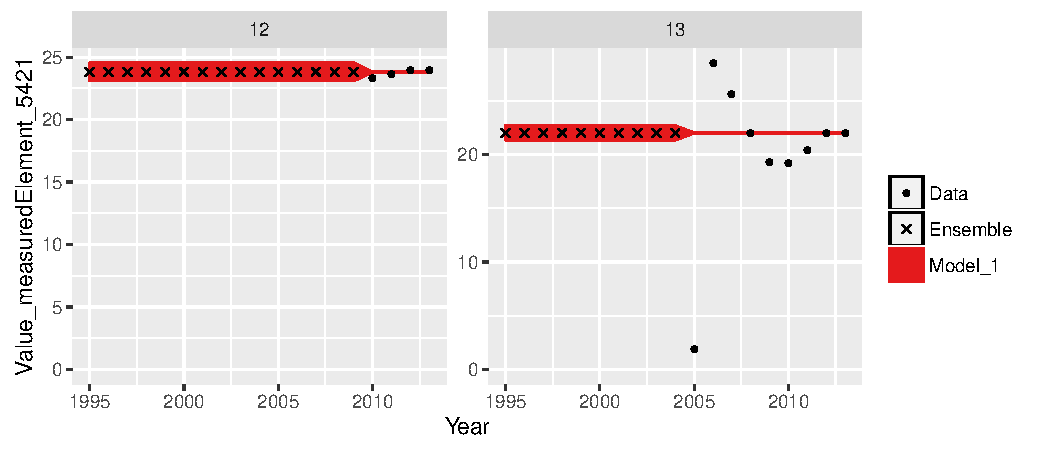
\includegraphics[width=\maxwidth]{figure/unnamed-chunk-18-1} 

}



\end{knitrout}

\subsection{defaultMixedModel}

The defaultMixedModel is a more complex model that's fit to global datasets
(rather than each individual time-series).  So, let's use a different dataset
to run some analyses with this model:

\begin{knitrout}
\definecolor{shadecolor}{rgb}{0.969, 0.969, 0.969}\color{fgcolor}\begin{kframe}
\begin{alltt}
\hlstd{mixedModelData} \hlkwb{=} \hlstd{okra[geographicAreaM49} \hlopt{<} \hlnum{100}\hlstd{, ]}
\hlcom{# mixedModelData = processProductionDomain(mixedModelData,}
\hlcom{#         processingParameters = defaultProcessingParameters())}
\hlstd{updateMissingFlags} \hlkwb{=} \hlkwa{function}\hlstd{(}\hlkwc{data}\hlstd{,} \hlkwc{value}\hlstd{,} \hlkwc{flag}\hlstd{,} \hlkwc{missingFlag} \hlstd{=} \hlstr{"M"}\hlstd{)\{}
    \hlstd{missingIndex} \hlkwb{=} \hlkwd{which}\hlstd{(}\hlkwd{is.na}\hlstd{(data[[value]]))}
    \hlkwd{invisible}\hlstd{(data[missingIndex,} \hlkwd{`:=`}\hlstd{(}\hlkwd{c}\hlstd{(flag),} \hlkwd{list}\hlstd{(missingFlag))])}
\hlstd{\}}
\hlkwd{updateMissingFlags}\hlstd{(}\hlkwc{data} \hlstd{= mixedModelData,} \hlkwc{value} \hlstd{=} \hlstr{"Value_measuredElement_5421"}\hlstd{,}
         \hlkwc{flag} \hlstd{=} \hlstr{"flagObservationStatus_measuredElement_5421"}\hlstd{)}
\end{alltt}
\end{kframe}
\end{knitrout}

Now, let's run the ensemble imputation with the default imputation parameters.
This example uses the \pkg{lme4} package to fit a mixed model.

\begin{knitrout}
\definecolor{shadecolor}{rgb}{0.969, 0.969, 0.969}\color{fgcolor}\begin{kframe}
\begin{alltt}
\hlstd{newParameters} \hlkwb{=} \hlkwd{defaultImputationParameters}\hlstd{(}\hlnum{5421}\hlstd{)}
\hlstd{newParameters}\hlopt{$}\hlstd{newImputationColumn} \hlkwb{=} \hlstr{"test"}
\hlstd{newParameters}\hlopt{$}\hlstd{estimateNoData} \hlkwb{=} \hlnum{TRUE}
\hlstd{model} \hlkwb{=} \hlkwd{ensembleModel}\hlstd{(}\hlkwc{model} \hlstd{= defaultMixedModel,} \hlkwc{extrapolationRange} \hlstd{=} \hlnum{Inf}\hlstd{,}
                      \hlkwc{level} \hlstd{=} \hlstr{"global"}\hlstd{)}
\hlstd{newParameters}\hlopt{$}\hlstd{ensembleModels} \hlkwb{=} \hlkwd{list}\hlstd{(model)}
\hlkwd{imputeVariable}\hlstd{(}\hlkwc{data} \hlstd{= mixedModelData,} \hlkwc{imputationParameters} \hlstd{= newParameters)}
\end{alltt}
\end{kframe}

{\centering 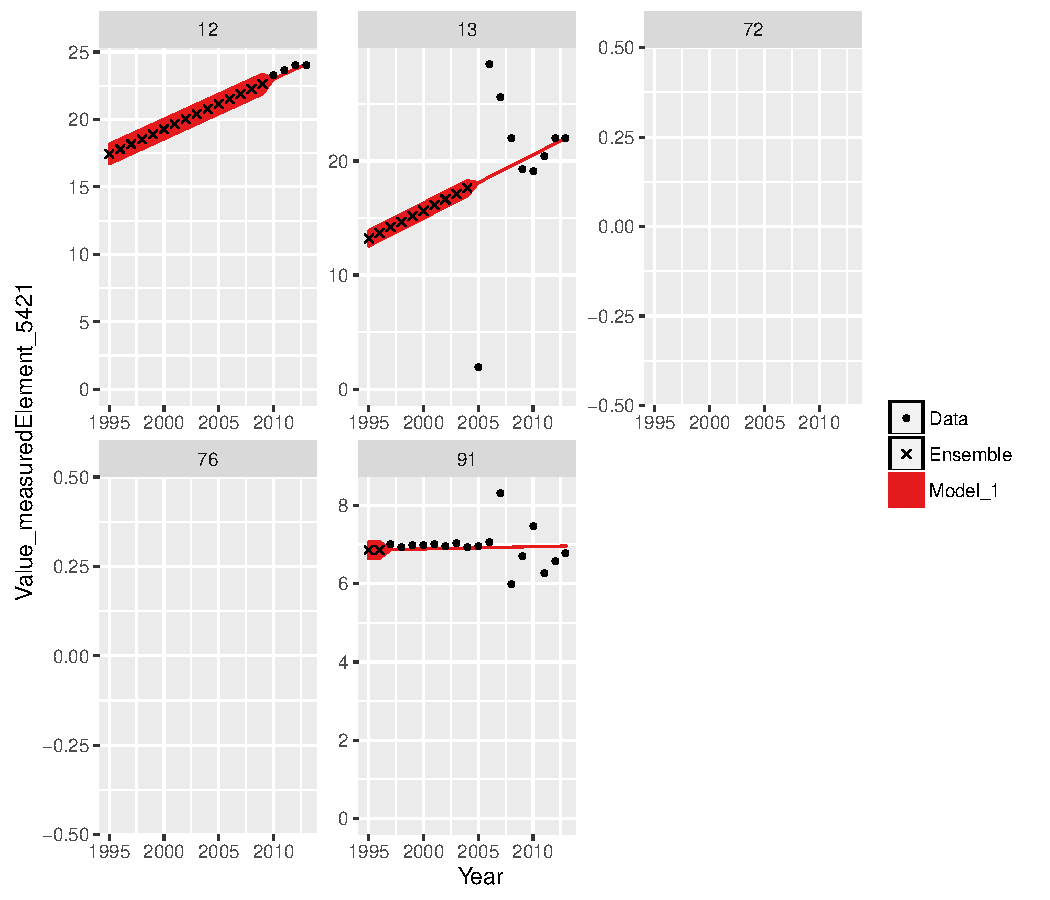
\includegraphics[width=\maxwidth]{figure/unnamed-chunk-20-1} 

}



\end{knitrout}

For most cases, we see the same results as we did with the linear regression: a
simple least-squares curve is fit to the available data and then that model is
used to impute the missing values.  However, the mixed model fit to the data
can also be used for estimation on time-series where very little data is
available, for example on area 46 and 66.

More complex cases are also available: for example, we could fit a hierarchical
model (also with the \pkg{lme4} package) that allows us to impute countries
with missing data based on some hierarchy (for example, continents).  In this
example, we just made up arbitrary regions.

\begin{knitrout}
\definecolor{shadecolor}{rgb}{0.969, 0.969, 0.969}\color{fgcolor}\begin{kframe}
\begin{alltt}
\hlkwd{invisible}\hlstd{(\{}
    \hlstd{mixedModelData[geographicAreaM49} \hlopt{==} \hlstr{"66"}\hlstd{, Value_measuredElement_5421} \hlkwb{:=} \hlnum{NA}\hlstd{]}
    \hlstd{mixedModelData[geographicAreaM49} \hlopt{==} \hlstr{"66"}\hlstd{,}
               \hlstd{flagObservationStatus_measuredElement_5421} \hlkwb{:=} \hlstr{"M"}\hlstd{]}
    \hlstd{mixedModelData[,region} \hlkwb{:=} \hlkwd{factor}\hlstd{(}\hlkwd{ifelse}\hlstd{(geographicAreaM49} \hlopt{<} \hlnum{15}\hlstd{,} \hlnum{1}\hlstd{,}
                                     \hlkwd{ifelse}\hlstd{(geographicAreaM49} \hlopt{<} \hlnum{50}\hlstd{,} \hlnum{2}\hlstd{,} \hlnum{3}\hlstd{)))]}
\hlstd{\})}
\hlkwd{formals}\hlstd{(defaultMixedModel)}\hlopt{$}\hlstd{modelFormula} \hlkwb{=} \hlstd{Value_measuredElement_5421} \hlopt{~}
    \hlstd{timePointYears}\hlopt{*}\hlstd{region} \hlopt{+} \hlstd{(timePointYears}\hlopt{|}\hlstd{geographicAreaM49}\hlopt{/}\hlstd{region)}
\hlstd{hierarchical} \hlkwb{=} \hlkwd{ensembleModel}\hlstd{(}\hlkwc{model} \hlstd{= defaultMixedModel,} \hlkwc{level} \hlstd{=} \hlstr{"global"}\hlstd{,}
                             \hlkwc{extrapolationRange} \hlstd{=} \hlnum{Inf}\hlstd{)}
\hlstd{globalMean} \hlkwb{=} \hlkwd{ensembleModel}\hlstd{(}\hlkwc{model} \hlstd{= defaultGlobalMean,} \hlkwc{level} \hlstd{=} \hlstr{"global"}\hlstd{,}
                           \hlkwc{extrapolationRange} \hlstd{=} \hlnum{Inf}\hlstd{)}
\hlstd{globalMedian} \hlkwb{=} \hlkwd{ensembleModel}\hlstd{(}\hlkwc{model} \hlstd{= defaultGlobalMedian,} \hlkwc{level} \hlstd{=} \hlstr{"global"}\hlstd{,}
                             \hlkwc{extrapolationRange} \hlstd{=} \hlnum{Inf}\hlstd{)}
\hlstd{newParameters}\hlopt{$}\hlstd{ensembleModels} \hlkwb{=} \hlkwd{list}\hlstd{(}\hlkwc{hierarchical} \hlstd{= hierarchical,}
                                    \hlkwc{globalMean} \hlstd{= globalMean,}
                                    \hlkwc{globalMedian} \hlstd{= globalMedian)}
\hlkwd{imputeVariable}\hlstd{(}\hlkwc{data} \hlstd{= mixedModelData,} \hlkwc{imputationParameters} \hlstd{= newParameters)}
\end{alltt}
\end{kframe}

{\centering 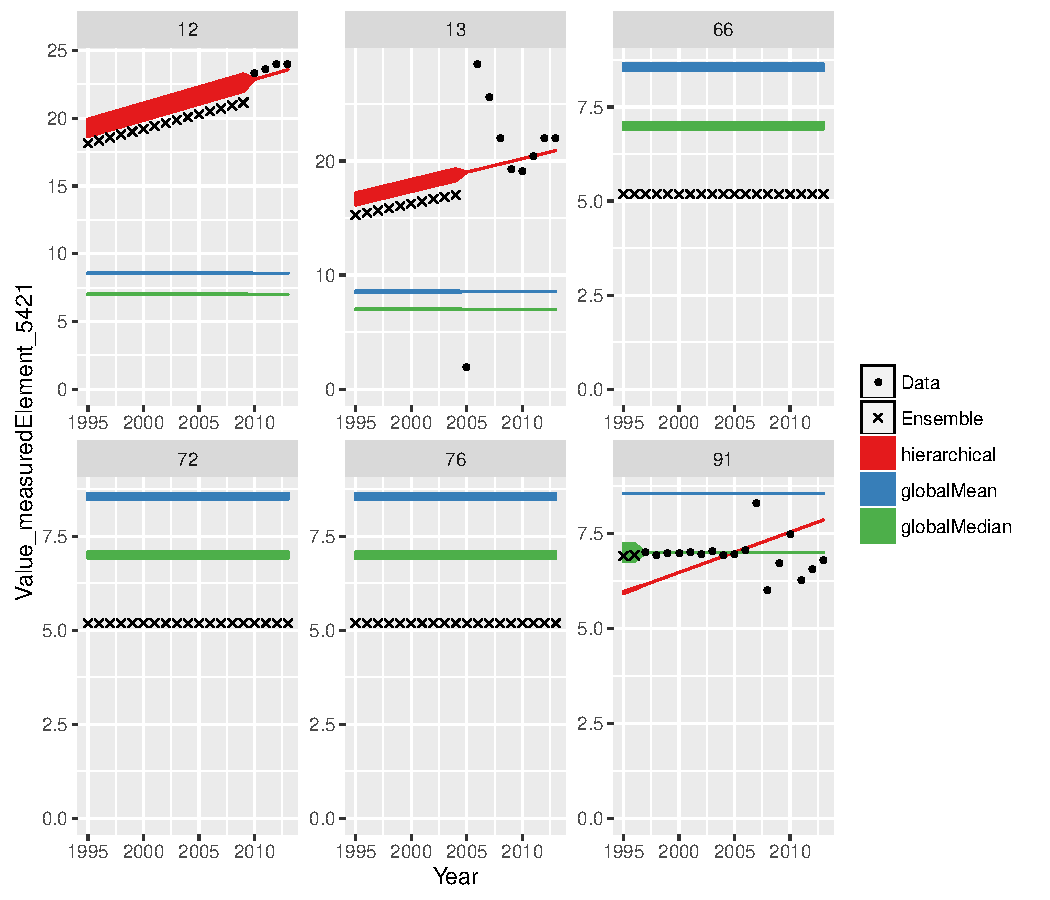
\includegraphics[width=\maxwidth]{figure/unnamed-chunk-21-1} 

}



\end{knitrout}

In this complicated example, we can see several different types of imputation
occurring.  The most common case seems to be the hierarchical model, which
simplifies to just a linear regression on countries with enough data to fit
the model.  The global mean and median don't seem to be as good of models, but
in a few cases they provide some value.

Note that we are also able to impute values in region 66, where no data exists
(because we deleted the one value that was present before we began).  This
imputation was performed by looking at the cross-validation error of the three
models considered on all the other datasets and averaging the error across all
available observations.  Generally the mixed model performs best, and so it
gets the most weight on this set of data where we have no available data.

\subsection{defaultNaive}

This model performs simple linear interpolation between available observations.
However, if a missing value is outside the range of the data, then this model
estimates that value by carrying back the first observation or carrying forward
the last observation (depending on if the missing value is before the available
data or after it).  Because of this, this model is not recommended for
extrapolation (and has a default extrapolationRange of 0 in allDefaultModels).

\begin{knitrout}
\definecolor{shadecolor}{rgb}{0.969, 0.969, 0.969}\color{fgcolor}\begin{kframe}
\begin{alltt}
\hlstd{model} \hlkwb{=} \hlkwd{ensembleModel}\hlstd{(}\hlkwc{model} \hlstd{= defaultNaive,} \hlkwc{extrapolationRange} \hlstd{=} \hlnum{0}\hlstd{,}
                      \hlkwc{level} \hlstd{=} \hlstr{"local"}\hlstd{)}
\hlstd{imputationParameters}\hlopt{$}\hlstd{ensembleModels} \hlkwb{=} \hlkwd{list}\hlstd{(model)}
\hlkwd{imputeVariable}\hlstd{(}\hlkwc{data} \hlstd{= exampleData,} \hlkwc{imputationParameters} \hlstd{= imputationParameters)}
\end{alltt}
\end{kframe}

{\centering 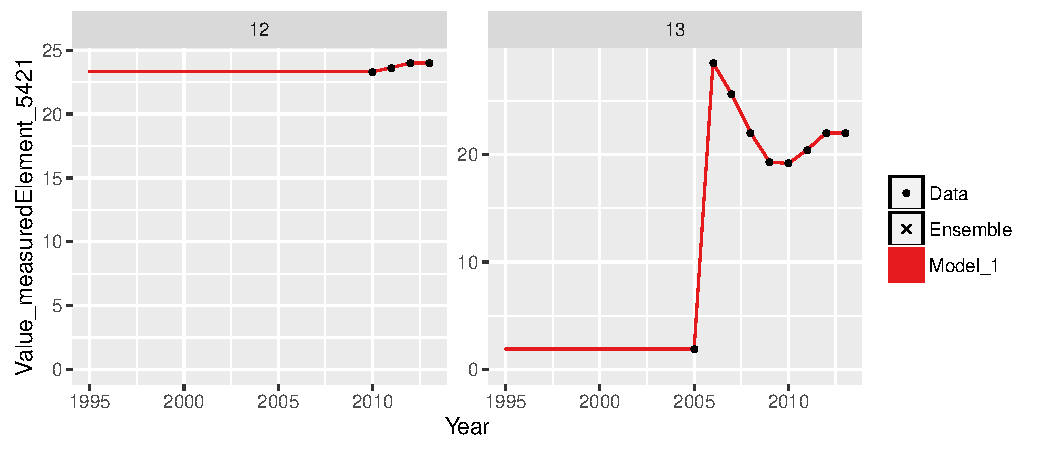
\includegraphics[width=\maxwidth]{figure/unnamed-chunk-22-1} 

}



\end{knitrout}

\subsection{defaultSpline}

The defaultSpline model uses the spline function from the stats package (part
of base) to fit a spline to the available observations.  Missing observations
are then imputed by the spline estimate at that location.

\begin{knitrout}
\definecolor{shadecolor}{rgb}{0.969, 0.969, 0.969}\color{fgcolor}\begin{kframe}
\begin{alltt}
\hlstd{model} \hlkwb{=} \hlkwd{ensembleModel}\hlstd{(}\hlkwc{model} \hlstd{= defaultSpline,} \hlkwc{extrapolationRange} \hlstd{=} \hlnum{0}\hlstd{,}
                      \hlkwc{level} \hlstd{=} \hlstr{"local"}\hlstd{)}
\hlstd{imputationParameters}\hlopt{$}\hlstd{ensembleModels} \hlkwb{=} \hlkwd{list}\hlstd{(model)}
\hlkwd{imputeVariable}\hlstd{(}\hlkwc{data} \hlstd{= exampleData,} \hlkwc{imputationParameters} \hlstd{= imputationParameters)}
\end{alltt}
\end{kframe}

{\centering 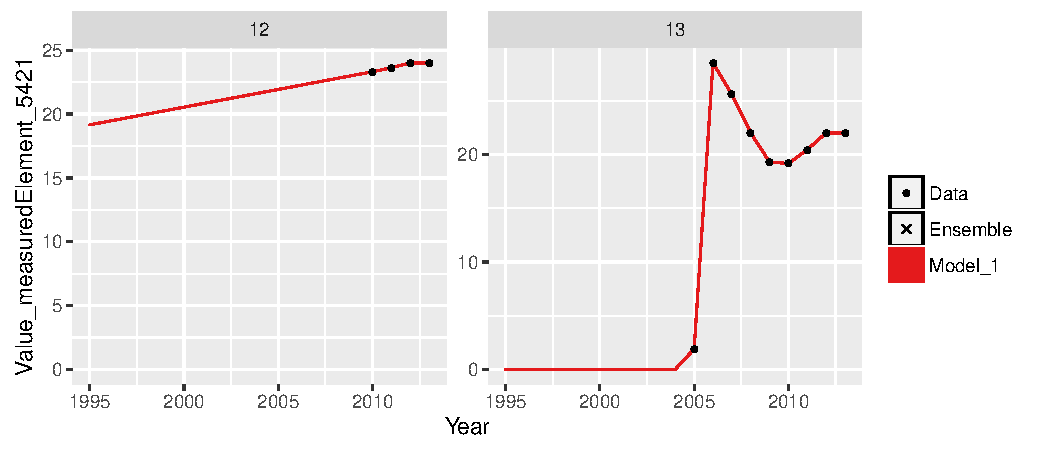
\includegraphics[width=\maxwidth]{figure/unnamed-chunk-23-1} 

}



\end{knitrout}

\end{document}
